% **************************************************************************************************************
% A Classic Thesis Style
% An Homage to The Elements of Typographic Style
%
% Copyright (C) 2007 Andr� Miede http://www.miede.de
%
% If you like the style then I would appreciate a postcard. My address
% can be found in the file ClassicThesis.pdf. A collection of the
% postcards I received so far is available online at
% http://postcards.miede.de
%
% License:
% This program is free software; you can redistribute it and/or modify
% it under the terms of the GNU General Public License as published by
% the Free Software Foundation; either version 2 of the License, or
% (at your option) any later version.
%
% This program is distributed in the hope that it will be useful,
% but WITHOUT ANY WARRANTY; without even the implied warranty of
% MERCHANTABILITY or FITNESS FOR A PARTICULAR PURPOSE.  See the
% GNU General Public License for more details.
%
% You should have received a copy of the GNU General Public License
% along with this program; see the file COPYING.  If not, write to
% the Free Software Foundation, Inc., 59 Temple Place - Suite 330,
% Boston, MA 02111-1307, USA.
%
% **************************************************************************************************************
% Note:
%    * You must not use "u etc. in strings/commands that will be spaced out (use \"u or real umlauts instead)
%    * Chapters must be marked with the \myChapter{Foo} command (sorry for the inconvenience at this point)
%    * New enumeration (small caps): \begin{aenumerate} \end{aenumerate}
%    * For margin notes: \graffito{}
%    * Do not use bold fonts in this style, it is designed around them
%    * Use tables as in the examples
%    * See classicthesis-ldpkg.sty for useful commands
% **************************************************************************************************************
% To Do:
%    * remove obsolete KOMA options and use \KOMAoptions instead
%    * support a List of Listings that looks like the other lists
% **************************************************************************************************************
%\documentclass[twoside,titlepage,fleqn,BCOR5mm]{scrbook}%,BCOR5mm

% Comentado por JCC 
\documentclass[10pt]{scrbook}%

%\usepackage[paperwidth=18.89cm,paperheight=24.58cm,twoside,bindingoffset=9mm,outer=2.2cm,inner=1cm,top=2.6cm,bottom=4.5cm]{geometry}

\let\upDelta\Delta
% ********************************************************************
% KOMA-Script setup (todo)
% ********************************************************************
\KOMAoptions{%
%    DIV=15,%
    BCOR=12mm,%
    %paper=b5,%
    fontsize=11pt,%
    cleardoublepage=empty,%
    headsepline=true,
    footinclude=true,%
    headinclude=true,%
    headlines=2.5,%
    open=right,%
    numbers=noenddot%
%    abstract=false%
}

\setlength{\paperwidth}{16.828cm} % set size for latex
\setlength{\paperheight}{26cm}
\special{papersize=16.828cm,26cm} % set size for ghostscript
\typearea[6mm]{1} % 6mm for spine

% ********************************************************************
% Development Stuff
% ********************************************************************
%\listfiles
%\usepackage[l2tabu, orthodox, abort]{nag}
%\usepackage[warning, all]{onlyamsmath}
% ********************************************************************
% Re-usable information
% ********************************************************************

% added by JCC to use Pygmentize 
% http://tex.stackexchange.com/questions/23458/how-to-install-syntax-highlight-package-minted-on-windows-7
% \newcommand\TestAppExists[3]{#2}
\usepackage{minted}


\newcommand{\myTitle}{INTELIGENCIA COMPUTACIONAL Y JUEGOS APLICADOS A LA ENSE\~NANZA\xspace}
\newcommand{\myDegree}{Doctor en Inform\'atica\xspace}
\newcommand{\myName}{Jos\'e Carpio Ca\~nada\xspace}
\newcommand{\myDegreeManualName}{Tesis Doctoral\xspace}
\newcommand{\myProf}{myProf\xspace}
\newcommand{\myOtherProf}{myOtherProf\xspace}
\newcommand{\myDirectorOne}{Juan Juli\'an Merelo Guerv\'os}
\newcommand{\myDirectorTwo}{V\'ictor Manuel Rivas Santos}
\newcommand{\myDirectorThree}{Alberto Prieto Espinosa}
\newcommand{\mySupervisor}{Prof. Dr. D. \myDirectorOne\\Prof. Dr. D. \myDirectorTwo}
\newcommand{\myFaculty}{Escuela T\'ecnica Superior de Inform\'atica y Telecomunicaciones\xspace}
\newcommand{\myDepartment}{Arquitectura y Tecnolog\'ia de Computadores\xspace}
\newcommand{\myDepartmentTwo}{Inform\'atica\xspace}
\newcommand{\myUni}{\protect{Universidad de Granada}\xspace}
\newcommand{\myUniTwo}{\protect{Universidad de Ja\'en}\xspace}
\newcommand{\myLocation}{Granada\xspace}
\newcommand{\myDay}{11}
\newcommand{\myTime}{Noviembre de 2015\xspace}

%*******************************************************
% Packages with options that might require adjustments
%*******************************************************
\usepackage[latin1]{inputenc}
\usepackage[spanish,american,english,es-nodecimaldot]{babel}
\usepackage[square,numbers,sort&compress]{natbib}
\usepackage[spanish]{babelbib}
\usepackage[T1]{fontenc}
\usepackage{textcomp}
\usepackage[mathcal]{euscript}
\usepackage{latexsym}
\usepackage{relsize}
%\usepackage{amsmath} %Incompatible con \usepackage{relsize}
\usepackage{amsfonts}
\usepackage{amssymb}
%\usepackage[sort]{cite}
\usepackage[right]{eurosym}
\usepackage[top]{mcaption}
\usepackage[margincaption]{sidecap}

\usepackage{colortbl}
\usepackage{multirow}
\usepackage{rotating}

\usepackage{lettrine}
\usepackage{textcase}

\usepackage{url}
\usepackage{caption}
\usepackage[tight,spanish]{minitoc}

\usepackage{calc}
\usepackage{fp}

\usepackage{pgfplots}
\usetikzlibrary{dateplot}

\usepackage{cmap}

\usepackage{ifthen}

\usepackage{fancyvrb} %FERGU
\usepackage{etex}
\usepackage{minted}
\usepackage{algorithmic}
\providecommand{\e}[1]{\ensuremath{\times 10^{#1}}}

%\usepackage[a4,frame,center]{crop} %,cross

\input{coloricos} %OJO CON ESTO (EVOSOFT) vs highlight.sty de SOA-SOCO
\usepackage[final]{listings}


% JCC
\usepackage{color}
\pagecolor{white}
\usepackage[final]{pdfpages}

% 
\usepackage[colorinlistoftodos,prependcaption,textsize=tiny]{todonotes}
%\newcommandx{\unsure}[2][1=]{\todo[linecolor=red,backgroundcolor=red!25,bordercolor=red,#1]{#2}}
%\newcommandx{\change}[2][1=]{\todo[linecolor=blue,backgroundcolor=blue!25,bordercolor=blue,#1]{#2}}
%\newcommandx{\info}[2][1=]{\todo[linecolor=OliveGreen,backgroundcolor=OliveGreen!25,bordercolor=OliveGreen,#1]{#2}}
%\newcommandx{\improvement}[2][1=]{\todo[linecolor=Plum,backgroundcolor=Plum!25,bordercolor=Plum,#1]{#2}}
%\newcommandx{\thiswillnotshow}[2][1=]{\todo[disable,#1]{#2}}
%


%\lstset{
%basicstyle=\ttfamily \scriptsize,
%backgroundcolor=\color{ultralightOrange},
%language=c++,
%frame=single,
%stringstyle=\ttfamily,
%showstringspaces=false
%} %DENTRO DE ESO HAY OTRO LISTINGS QUE SE COME LO DE ARRIBA, PERO NO SE SI AFECTA OTRAS COSAS...
%*******************************************************
\usepackage{classicthesis-ldpkg}
%*******************************************************
% Options for classicthesis.sty:
% tocaligned eulerchapternumbers drafting linedheaders listsseparated
% subfigure nochapters beramono eulermath parts minionpro pdfspacing
\usepackage[pdfspacing,eulerchapternumbers,crownquartopaper,%drafting,%linedheaders,%tocaligned,%
            subfigure,beramono,eulermath,parts]{classicthesis2}
% ********************************************************************
% Language/strings for backrefs (change here, thanks, Lorenzo)
%*******************************************************
\renewcommand{\backrefnotcitedstring}{\relax}%(Not cited.)
% Elimina todas estas cosas que est�n comentadas, no hacen m�s que
% estorbar - JJ 
%\renewcommand{\backrefcitedsinglestring}[1]{(Citado en la p\'agina~#1.)}
%\renewcommand{\backrefcitedmultistring}[1]{(Citado en las p\'aginas~#1.)}
%\renewcommand{\backreftwosep}{ y~}
%\renewcommand{\backreflastsep}{ y~}
% ********************************************************************
% Setup and Finetuning
%*******************************************************
\newlength{\abcd} % for ab..z string length calculation
\newcommand{\myfloatalign}{\centering} % how all the floats will be aligned
\setlength{\extrarowheight}{3pt} % increase table row height
% ********************************************************************
% Captions look and feel
%*******************************************************
\DeclareCaptionFont{titlecolor}{\color{titlecolor}\fontfamily{pbk}\selectfont}
\DeclareCaptionFont{alternateTitlecolor}{\color{alternateTitlecolor}\fontfamily{pbk}\selectfont}
\captionsetup{justification=RaggedRight,format=plain,labelsep=newline,font=scriptsize,labelfont=titlecolor,textfont=alternateTitlecolor}%
% ********************************************************************
% Where to look for graphics
%*******************************************************
%\graphicspath{{gfx/}{misc/}} % considered harmful according to l2tabu
% ********************************************************************
% Hyperreferences
%*******************************************************
\hypersetup{%
    colorlinks=true, linktocpage=true, pdfstartpage=3, pdfstartview=FitV,%
    breaklinks=true, pdfpagemode=UseNone, pageanchor=true, pdfpagemode=UseOutlines,%
    plainpages=false, bookmarksnumbered, bookmarksopen=true, bookmarksopenlevel=1,%
    hypertexnames=true, pdfhighlight=/O,%hyperfootnotes=true,%nesting=true,%frenchlinks,%
    urlcolor=colorCorporativoOscuro, linkcolor=alternateTitlecolor, citecolor=Maroon, %pagecolor=RoyalBlue,%
    % uncomment the following line if you want to have black links (e.g., for printing)
    %urlcolor=Black, linkcolor=Black, citecolor=Black, %pagecolor=Black,%
    pdftitle={\myTitle},%
    pdfauthor={\textcopyright\ \myName, \myUni, \myFaculty},%
    pdfsubject={},%
    pdfkeywords={},%
    pdfcreator={pdfLaTeX},%
    pdfproducer={LaTeX with hyperref and classicthesis}%
}
%********************************************************************
% Hyphenation
%*******************************************************
%\hyphenation{Mul-ti-pli-ca-ti-ve de-sa-rro-llar he-te-ro-g�-ne-os pro-pues-ta o-fi-ci-na vi-de-o-ga-mes zoo-kee-per sub-po-pu-la-tion pa-ra-digm Sprin-ger Mi-guel Mo-ra ha-bi-ta-ci�n I-lle-ras Ge-ne-bot pre-sents Ba-ye-sian al-go-rithms E-C-F re-pla-cer re-pla-cer-Na-me He-Ha OS-Gi OS-Gi-Liath W-S-D-L pro-vi-der M-M-D-P}


%********************************************************************
% Redefinir en espa�ol la edici�n en la bibliograf�a
%*******************************************************

\declarebtxcommands{spanish}{%
\def\btxnumeralshort#1{%
${#1}^a$}%\btxnumeralfallback{spanish}{#1}}%
\def\btxnumerallong#1{%
${#1}^a$}%\btxnumeralfallback{spanish}{#1}}%
}

%********************************************************************
% Renombrar al espa�ol algunos identificadores
%*******************************************************

%\renewcommand{\contentsname}{Lista de Contenidos}
%\renewcommand{\listfigurename}{Lista de Figuras}
%\renewcommand{\listtablename}{Lista de Tablas}
%\renewcommand{\bibname}{Bibliograf\'ia}
%\renewcommand{\partname}{Parte}
%\renewcommand{\figurename}{Figura}
%\renewcommand{\tablename}{Tabla}
%\newcommand{\tablaname}{Tabla}
%\renewcommand{\cfttabpresnum}{\tablaname~}

\renewcommand{\person}[1]{{\color{Maroon}{#1}}}

\selectbiblanguage{spanish}

%\renewcommand{\spacedallcaps}[1]{\textsc{\MakeTextUppercase{#1}}}
%\renewcommand{\spacedlowsmallcaps}[1]{\textsc{\MakeTextUppercase{#1}}}

%********************************************************************
% Tipos de letras
%*******************************************************

%\renewcommand{\encodingdefault}{T1}
%\renewcommand{\familydefault}{gm}%papyrus}%bradley} %pbk,ppl
%\renewcommand{\seriesdefault}{b}

%\renewcommand{\rmdefault}{bradley}

\newcommand{\Copyright}{{\small$^\mathrm{\copyright}$}~}
\newcommand{\apriori}{\emph{a priori}\xspace}
\newcommand{\aposteriori}{\emph{a posteriori}\xspace}
\newcommand{\etal}{\emph{et al.}\xspace}
\newcommand{\cronbach}{\mbox{$\alpha$--\emph{Cronbach}}\xspace} % �Esto te sirve para algo? - JJ 

\newcommand{\itemlabel}[1]{{\color{Maroon}{\textsc{#1}}}}

\newcommand{\mysize}{\tiny}

%********************************************************************
% Colores
%*******************************************************

%\definecolor[named]{ultralightOrange}{rgb}{1,.94,.72}
%\definecolor[named]{highlightOrange}{rgb}{1,.86,.29}
%\definecolor[named]{lightOrange}{rgb}{1,.45,0}
\definecolor[named]{darkOrange}{rgb}{.8,.3,0}

\definecolor[named]{minimumOrange}{rgb}{1,.976,.474}
\definecolor[named]{ugrOrange}{rgb}{.945,.365,.165} % PANTONE 179: {R:241, G:93, B:42}
%\definecolor[named]{ugrOrange}{cmyk}{0,.309,.368,0} % PANTONE 179: {C:0, M:79, Y:94, K:0}
\definecolor[named]{ugrGray}{rgb}{.463,.482,.494}

%\definecolorseries{ugrOrangeSerie}{rgb}{last}{ugrOrange}{white}
%\resetcolorseries[10]{ugrOrangeSerie}

\colorlet{ultralightOrange}{ugrOrange!5!minimumOrange}
\colorlet{highlightOrange}{ugrOrange!25!minimumOrange}
\colorlet{lighterOrange}{ugrOrange!40!minimumOrange}
\colorlet{lightOrange}{ugrOrange!75!minimumOrange}

\definecolor{colorCorporativoMasSuave}{named}{ultralightOrange}
\definecolor{colorCorporativoSuave}{named}{highlightOrange}
\definecolor{colorCorporativoMedioSuave}{named}{lighterOrange}
\definecolor{colorCorporativoMedio}{named}{lightOrange}
\definecolor{colorCorporativo}{named}{ugrOrange}
\definecolor{colorCorporativoOscuro}{named}{darkOrange}
\definecolor{Maroon}{named}{colorCorporativoOscuro}

\definecolor{headColor}{named}{white}%{colorCorporativoMasSuave}
\definecolor{titleNumbercolor}{named}{ugrGray}
\definecolor{titlecolor}{named}{ugrOrange}
\definecolor{alternateTitlecolor}{named}{darkOrange}

\newcolumntype{A}{%
>{\color{black}\columncolor{colorCorporativoSuave}}%
p{0.95\textwidth}}

\newcolumntype{B}{%
>{\color{black}\columncolor{colorCorporativoMasSuave}}%
p{0.95\textwidth}}

\newcolumntype{C}{%
>{\columncolor{colorCorporativoSuave}}p{\textwidth}}
%>{\columncolor{colorCorporativo}}p{4pt}}

\newcolumntype{D}{%
>{\color{black}\fontfamily{pbk}\selectfont\columncolor{colorCorporativoSuave}}p{8em}}
%>{\columncolor{colorCorporativo}}p{4pt}

%********************************************************************
% Cabeceras
%*******************************************************

% Mini tablas de contenidos. Paquete minitoc
%\def\ptctitle{Index}
%\def\mtctitle{Index}
%\def\stctitle{Index}
\def\ptctitle{\'Indice}
\def\mtctitle{\'Indice}
\def\stctitle{\'Indice}
\setlength{\mtcindent}{0pt}
\renewcommand{\mtifont}{\normalsize\scshape\lsstyle}

%\typearea[current]{last}
%\typearea[current]{current}
%\setlength{\topmargin}{-4em}
%\setlength{\textheight}{590.80026pt}%{595.80026pt}
%\setlength{\tabcolsep}{1em}




\newboolean{TesisCompleta}
\setboolean{TesisCompleta}{false}

\newboolean{PaginasDeInicio}
\setboolean{PaginasDeInicio}{true}

\newcounter{IncluyeCapitulo}
\setcounter{IncluyeCapitulo}{2}

% \includeonly{Chapters/01-introduccion}

% ********************************************************************
% ********************************************************************
% ********************************************************************
% Comienza el documento
% ********************************************************************
% ********************************************************************
% ********************************************************************
\begin{document}

\frenchspacing
\raggedbottom
%\selectlanguage{spanish}
%\renewcommand{\contentsname}{Lista de Contenidos}
%\renewcommand{\listfigurename}{Lista de Figuras}
%\renewcommand{\listtablename}{Lista de Tablas}
%\renewcommand{\bibname}{Bibliograf\'ia}
%\renewcommand{\partname}{Parte}
%\renewcommand{\figurename}{Figura}
%\renewcommand{\tablename}{Tabla}
%\renewcommand{\figureautorefname}{Figura}
%\renewcommand{\tableautorefname}{Tabla}
%\renewcommand{\paragraphautorefname}{P\'arrafo}
%\renewcommand{\subparagraphautorefname}{Subp\'arrafo}
%\renewcommand{\footnoteautorefname}{Nota al pie}
%\renewcommand{\FancyVerbLineautorefname}{}
%\renewcommand{\theoremautorefname}{Teorema}
%\renewcommand{\appendixautorefname}{Ap\'endice}
%\renewcommand{\equationautorefname}{Ecuaci\'on}
%\renewcommand{\itemautorefname}{Item}
%\newcommand*{\subfigureautorefname}{Figura}

% Par�metros para Lettrine (lo de la primera letra m�s grande en los comienzos de los cap�tulos)
%
\setcounter{DefaultLines}{2}
\renewcommand{\DefaultLoversize}{0.1} %0.25
\renewcommand{\DefaultLraise}{0.3} %0.25
\renewcommand{\DefaultLhang}{0.5} %0.5
\setlength{\DefaultFindent}{0pt}%0.5em}
\setlength{\DefaultNindent}{0pt}%0.1em}
\setlength{\DefaultSlope}{0pt}
\renewcommand{\LettrineFontHook}{\color{colorCorporativoOscuro}\fontfamily{fau}}%{fau}pzc}\fontseries{bx}\fontshape{it}}
\renewcommand{\LettrineTextFont}{\color{colorCorporativoOscuro}\fontfamily{fau}\scshape}
\renewcommand\listfigurename{Lista de Figuras}
\renewcommand\listtablename{Lista de Tablas}
\renewcommand\contentsname{Tabla de Contenidos}
\renewcommand\appendixname{Ap\'endice}
\renewcommand\bibname{Referencias}
\renewcommand{\partname}{Parte}
\renewcommand{\indexname}{Indice}
\renewcommand{\figurename}{Figura}
\renewcommand{\tablename}{Tabla}
\renewcommand{\figureautorefname}{Figura}
\renewcommand{\tableautorefname}{Tabla}
\renewcommand{\paragraphautorefname}{P\'arrafo}
\renewcommand{\subparagraphautorefname}{Subp\'arrafo}
\renewcommand{\footnoteautorefname}{Nota al pie}
%\renewcommand{\FancyVerbLineautorefname}{}
\renewcommand{\theoremautorefname}{Teorema}
\renewcommand{\appendixautorefname}{Ap\'endice}
\renewcommand{\equationautorefname}{Ecuaci\'on}
%\renewcommand{\itemautorefname}{Item}
% \newcommand*{\subfigureautorefname}{Figura}

\pagenumbering{roman}
\pagestyle{scrheadings}%{plain}

\renewcommand{\labelenumii}{\arabic{enumii}.}

% JCC fuerza un salto de linea dentro de la celda de una tabla
\newcommand{\specialcell}[2][c]{%
  \begin{tabular}[#1]{@{}c@{}}#2\end{tabular}}

  
  

%********************************************************************
% Definiciones Captions
%*******************************************************

\sidecaptionvpos{figure}{t}

\ifthenelse{\boolean{PaginasDeInicio}}{
%********************************************************************
% Frontmatter
%*******************************************************



% \include{FrontBackmatter/DirtyTitlepage}
\pagecolor{white}
\pdfbookmark[1]{Portada}{Portada}
%*******************************************************
% Signed Titlepage 
%*******************************************************
\begin{titlepage}
    \begin{center}
        \large
        \vspace*{1.5cm}
        \includegraphics[width=8cm]{gfx/ugr_formal} \\

        \vspace{1.5cm}

        {\color{ugrOrange}\spacedallcaps{\myTitle}} \\ \bigskip
	{\textcolor{ugrGray} {\small Presentado por}} \\ \bigskip
        \spacedlowsmallcaps{\myName}

        \vspace{1.5cm}
\textcolor{ugrGray}
        {\small To apply for the }\normalsize\\
        \large\spacedlowsmallcaps{International PhD Degree in} \\ 
        \large\spacedlowsmallcaps{Computer and Network Engineering} \\
\vspace{1.5cm}
\textcolor{ugrGray}{\small Directores }\normalsize\\
        \large\spacedlowsmallcaps{\myDirectorOne}\\
        \large\spacedlowsmallcaps{\myDirectorTwo}\\
        \vspace{3cm}

        {\small Firmado: \myName }\\ \bigskip
	Noviembre 2014


    \end{center}
\end{titlepage}   
%\include{FrontBackmatter/Titlepage}
\include{FrontBackmatter/Titleback}
\cleardoublepage
%%*******************************************************
% Signed Titlepage 
%*******************************************************
\begin{titlepage}
    \begin{center}
        \large
        \vspace*{1.5cm}
        \includegraphics[width=8cm]{gfx/ugr_formal} \\

        \vspace{1.5cm}

        {\color{ugrOrange}\spacedallcaps{\myTitle}} \\ \bigskip
	{\textcolor{ugrGray} {\small Presentado por}} \\ \bigskip
        \spacedlowsmallcaps{\myName}

        \vspace{1.5cm}
\textcolor{ugrGray}
        {\small To apply for the }\normalsize\\
        \large\spacedlowsmallcaps{International PhD Degree in} \\ 
        \large\spacedlowsmallcaps{Computer and Network Engineering} \\
\vspace{1.5cm}
\textcolor{ugrGray}{\small Directores }\normalsize\\
        \large\spacedlowsmallcaps{\myDirectorOne}\\
        \large\spacedlowsmallcaps{\myDirectorTwo}\\
        \vspace{3cm}

        {\small Firmado: \myName }\\ \bigskip
	Noviembre 2014


    \end{center}
\end{titlepage}   

%\cleardoublepage
%*******************************************************
% Declaration
%*******************************************************
\refstepcounter{dummy}
\pdfbookmark[1]{Visto Bueno}{Visto Bueno}
\chapter*{Visto Bueno}
\thispagestyle{empty}
\bigskip

%\noindent\textit{\myLocation, \myTime}

\vfil

El \textbf{Prof. Dr. D. \myDirectorOne}, Catedr�tico de Universidad del Departamento de \myDepartment de la \myUni y el profesor \textbf{Prof. Dr. D. \myDirectorTwo}, Titular de Universidad del Departamento de \myDepartmentTwo de la \myUniTwo,

\bigskip

\textsc{certifican:}

\bigskip

\noindent Que la memoria titulada:
\begin{center}
``\textbf{\emph{\myTitle}}''
\end{center}
ha sido realizada por \textbf{D. \myName} bajo nuestra direcci�n en el Departamento de \myDepartment de la \myUni para optar al grado de \textbf{\myDegree}.

\vfil

\begin{center}
En \myLocation, a \myDay\xspace de \myTime.
\end{center}
\vfil
Los Directores de la tesis doctoral:\\
\vspace{2cm}

\begin{center}
Fdo. \myDirectorOne \\ y \myDirectorTwo \\
\end{center}

% \begin{flushright}
%     \begin{tabular}{m{5cm}}
%         \\ \hline
%         \centering\myName \\
%     \end{tabular}
% \end{flushright}

\cleardoublepage
%*******************************************************
% Declaration
%*******************************************************
\refstepcounter{dummy}
\pdfbookmark[1]{Declaraci�n}{Declaraci�n}
\chapter*{Declaraci�n}
\thispagestyle{empty}
\vfill

\noindent El doctorando \myName y los directores de la tesis \myDirectorOne y \myDirectorTwo \xspace garantizamos, al firmar esta tesis doctoral, que el trabajo ha sido realizado por el doctorando bajo la direcci�n de los directores de la tesis y hasta donde nuestro conocimiento alcanza, en la realizaci�n del trabajo, se han respetado los derechos de otros autores a ser citados, cuando se han utilizado sus resultados o publicaciones.  
\smallskip


\bigskip

\noindent\textit{\myLocation, \myTime}

\bigskip
\bigskip
\bigskip

\begin{flushright}
    \begin{tabular}{m{3cm}m{7cm}}
        & \\ \hline
        \centering\myName & \myDirectorOne \newline y \myDirectorTwo
    \end{tabular}
\end{flushright}

\vfill
\cleardoublepage
%*******************************************************
% Dedication
%*******************************************************
\thispagestyle{empty}
%\phantomsection
\refstepcounter{dummy}
\pdfbookmark[1]{Dedicatoria}{Dedicatoria}

\vspace*{3cm}

\begin{flushright}
A mi familia: \hspace{3em}\\
Manuel Angel, Matilde, Manuel Jos�, Fernando, Lolita y Elisa Matilde.\\
\end{flushright}



\medskip

\cleardoublepage
%*******************************************************
% Abstract
%*******************************************************
%\renewcommand{\abstractname}{Abstract}
\pdfbookmark[1]{Abstract}{Abstract}
\begingroup
\let\clearpage\relax
\let\cleardoublepage\relax
\let\cleardoublepage\relax



\pdfbookmark[1]{Abstract}{Abstract}
\chapter*{Abstract}

% The objective of this thesis is to prove that the Service Oriented Architecture (SOA) paradigm can be used to create distributed, heterogeneous, dynamic and standards-based environments for Evolutionary Algorithms (EAs). SOA provides independence in programming language and transmission mechanisms, and also facilitates  dynamic component management. 

% A methodology to develop EAs in these environments is proposed. In this methodology, called SOA-EA, the SOA paradigm is proposed to develop Service Oriented Evolutionary Algorithms (SOEAs).  The proposed methodology takes into account the requirement to develop services and EAs, and it provides the steps to identify, specify, implement and deploy the elements that conform a SOEA, and how to convert a traditional EA into a SOEA. To validate this methodology, it has been used to create a framework for SOEAs, called OSGiLiath, based in a public specification technology (OSGi). This framework provides mechanisms for dynamic component management and language and transmission independence. 

% OSGiLiath and SOA-EA have been used to carry out experiments in different areas to validate dynamic control and different and heterogeneous environments: decentralized distributed EAs, other systems integration and different EA models.


\chapter*{Resumen}
%Esta Tesis Doctoral trata de probar que usar un marco determinado es
%el m�s adecuado para solucionar problemas actuales en los Algoritmos

% aparte de que no se entiende, est� mal: usar un marco... es el m�s
% adecuado �Qu� marco? �Sabes cu�l? �Lo vas a buscar en la tesis? �Vas
% a comparar varios marcos? Si lo sabes de antemano, di cual y por qu�
% a priori debe ser el m�s adecuado - JJ
%Evolutivos en desarrollo, integraci�n, interoperabilidad y
%dinamismo. Para validar este objetivo la tesis se ha dividido en 3
%partes.  
% Yo quitar�a desarrollo; para desarrollar los lenguajes de script son
% m�s f�ciles - JJ

%Primero se analizan las nuevas tendencias % las tendencias no se
                                % analizan, se hallan. �Esto d�nde lo
                                % haces? Ten en cuenta que toda la
                                % tesis debe de ir a avanzar estos
                                % tres objetivos, y *debes decirlo
                                % expl�citamente* - JJ
%en investigaci�n en Algoritmos Evolutivos para detectar sus principales carencias y se propone el uso de Arquitectura Orientada a Servicios (AOS) como el marco para resolver estas carencias.

%La siguiente parte de esta tesis propone una metodolog�a (SOA-EA) para
%desarrollar Algoritmos Evolutivos Orientados a Servicios (AEOS). Esta
%metodolog�a se ha utilizado para implementar un framework para AEOS,
%llamado OSGiLiath, utilizando una tecnolog�a concreta (OSGi). Se
%presentan diferentes experimentos para validar cada una de las mejoras
%propuestas. % �Qu� mejoras? �El objetivo de la tesis son esas mejoras?
            % No has mencionado ni una vez si has tenido que hacer un
            % cambio en el algoritmo ni si has propuesto un nuevo
            % algoritmo. �La adaptaci�n de los AGs a OSGi es directa?
            % Si es as�, es s�lo implementaci�n y no hay mucha
            % tesis. �Tienen m�s enjundia?

%OSGiLiath se ha usado tambi�n para desarrollar un m�todo para adaptar
%el tama�o de poblaci�n de un AE distribuido a la potencia de calculo
%de los nodos que forman el sistema distribuido. Finalmente, SOA-EA y
%OSGiLiath se han utilizado en otras aplicaciones: generaci�n de un bot
%inteligente para un juego en tiempo real y arte generativo. % �Eh? �Se
                                % ha usado tambi�n? �Te pillaba de
                                % camino? �Es parte de la tesis? �Es
                                % consecuencia de la tesis? �La
                                % prueba? �En esas aplicaciones se
                                % prueba que es el m�s guay o te
                                % pillaban de camino? - JJ

%Esto es lo que deber�as haber escrito para empezar y no perderlo
%nunca de vista. �C�mo puedes escribir la tesis si no sabes lo que
%pretende? - JJ FERGU: estaba en el github, pero lo pongo aqu� (luego lo traduzco cuando tenga el visto bueno)

\vfill

% No me gusta nada este resumen. No abarca toda la tesis (no abarca
% las aplicaciones ni las encaja m�s que con un "tambi�n". 
%FERGU: reescrito abajo entero

% El objetivo de esta tesis es demostrar que el paradigma de Arquitectura Orientada a Servicios (AOS) puede usarse para crear entornos distribuidos, heterog�neos, din�micos y basados en est�ndares para Algoritmos Evolutivos (AEs). AOS proporciona independencia en el lenguaje de programaci�n y mecanismo de transmisi�n y facilita la administraci�n de componentes de forma din�mica. 

% Se propone crear una metodolog�a para desarrollar AEs en estos entornos. En esta metodolog�a, denominada SOA-EA, se propone el uso del paradigma de SOA para desarrollar Algoritmos Evolutivos Orientados a Servicios (AEOS).  La metodolog�a propuesta tiene en cuenta los requisitos para desarrollar servicios y EAs y proporciona los pasos para identificar, especificar, implementar y desplegar los componentes que forman un AEOS, y c�mo convertir un AE tradicional a un AEOS. Para validarla, esta metodolog�a se ha utilizado para crear un framework para AEOS, llamado OSGiLiath, basado una tecnolog�a p�blica (OSGi). Este framework  proporciona mecanismos para administraci�n de componentes din�micos, independencia del lenguaje y protocolo de comunicaci�n. 

% Tanto OSGiLiath como SOAEA se han utilizado para realizar experimentos en distintos campos para validar el control del dinamismo y la heterogeneidad: AEs distribuidos no centralizados, integraci�n con otros sistemas y distintos modelos de EAs.

\endgroup

\vfill
\cleardoublepage
% JCC
% %*******************************************************
% Publications
%*******************************************************
\pdfbookmark[1]{Publications}{Scientific Publications}
\chapter*{Scientific Publications}
Some of the ideas, images and data exposed in this thesis have been previously published in the next references:
\bigskip

\begin{itemize}
% \item \person{Pablo Garc�a-S�nchez, J. Gonz�lez, Pedro A. Castillo, Maribel Garc�a Arenas, Juan Juli�n Merelo Guerv�s} \emph{Service oriented evolutionary algorithms}.  Soft Comput. 17(6): 1059--1075 (2013).


% no metas estos del "companion", que todos sabemos lo que es... 

% \item \person{Pablo Garc�a-S�nchez, Maria I. Garc�a Arenas, Antonio Miguel Mora, Pedro A. Castillo, Carlos Fernandes, Paloma de las Cuevas, Gustavo Romero, Jes�s Gonz�lez, Juan Juli�n Merelo Guerv�s} \emph{ Developing services in a service oriented architecture for evolutionary algorithms}. In Proceeding of the fifteenth annual conference companion on Genetic and evolutionary computation conference companion. ACM, 2013. p: 1341-1348.

% \item \person{Pablo Garc�a-S�nchez} \emph{ A service oriented evolutionary architecture: applications and results}. In Proceeding of the fifteenth annual conference companion on Genetic and evolutionary computation conference companion. ACM, 2013. p: 1663--1666.

% \item \person{Pablo Garc�a-S�nchez, J. Gonz�lez, Pedro A. Castillo, Juan Juli�n Merelo Guerv�s, Antonio Miguel Mora, Juan Lu�s Jim�nez Laredo, Maribel Garc�a Arenas} \emph{ A Distributed Service Oriented Framework for Metaheuristics Using a Public Standard}. In Proceeding of Nature Inspired Cooperative Strategies for Optimization. Studies in Computational Intelligence. Springer, 2010. p: 211--222.


% \item \person{P. Garc�a-S�nchez, A. Fern�ndez-Ares, A. M. Mora, P. A. Castillo, J. Gonz�lez and J.J. Merelo} \emph{Tree depth influence in Genetic Programming for generation of competitive agents for RTS games}. Applications of Evolutionary Computation, EvoApplicatons 2010: EvoCOMPLEX, EvoGAMES, EvoIASP, EvoINTELLIGENCE, EvoNUM, and EvoSTOC, Proceedings. Springer, 2014. Lecture Notes in Computer Science (to appear).

% \item \person{P. Garc�a-S�nchez, A. M. Mora, P. A. Castillo, J. Gonz�lez and J.J. Merelo} \emph{A methodology to develop Service Oriented Evolutionary Algorithms}. Proceedings of 8th International Symposium on Intelligent Distributed Computing (IDC'2014) Springer, 2014. Studies in Computational Science (to appear).

\end{itemize}

\cleardoublepage
%*******************************************************
% Acknowledgments
%*******************************************************
\pdfbookmark[1]{Agradecimientos}{agradecimientos}

\begin{flushright}
 
\end{flushright}



\bigskip

\begingroup
\let\clearpage\relax
\let\cleardoublepage\relax
\let\cleardoublepage\relax
\chapter*{Agradecimientos}
Mis agradecimientos van en primer lugar a mi familia Manuel Jos�, Matilde, Manuel �ngel, Fernando, Lola y Elisa que son las ramitas que dan fuerza 
y sentido a la vida.
A JJ y V�ctor, por su paciencia, por dejar que me equivocase tantas veces y sobre todo por haber sido capaces de darme la �ltima oportunidad despu�s
 de tantas anteriores.   
A Nicol�s, Carmen, Alicia, Nico y Eloy que ha sido mi segunda familia durante las estancias en el CITIC por su apoyo, sus risas matutinas, sus consejos
 y sus maravillosas cenas.
A mis compa�eros de Geneura que me acompa�aron en este largo viaje JJ, V�ctor, Pedro, Gustavo, Pablo, Juanlu, Antonio Mora, Maribel, Paloma, Antares a
 los que espero poder devolver alg�n d�a todo lo que me han dado. A mis compa�eros de Huelva, Nacho, Miguel �ngel, Fran, Gonzalo, Manuel, Manuel Emilio, 
 Manolo Vasallo, Teresa, Jos� Luis �lvarez, Jos� Luis Arjona, Paco M�rquez, Patricia, I�aki, Nieves, Antonio Peregr�n, Manolo Redondo, Javier Aroba por
 las maravillosas charlas sobre temas cient�ficos y no cient�ficos. A Jos� Manuel And�jar por apostar por mi desde el principio y por dejarme meter la
 pata. A los compa�eros de Simple LAB Juan Diego, Manuel, Miguel �ngel, Juan Manuel Enrique y Antonio por tanta energ�a e ilusi�n puesta en los nuevos
 proyectos. A la gente de CRM y en especial a Antonio Palanco y su familia por estar siempre dispuesto a echar un cable para lo que sea. 
A Carmen, Cristina, Fernando y todos los que colaboraron en hacer que la FLL se celebrase en Huelva por primera y segunda vez.   
A los compa�eros y personal del CITIC por hacer de ese espacio un hogar para muchos investigadores.  Al Dr. Tom�s Mateo Sanguino sin cuyo trabajo y tes�n
 no hubiese sido posible esta tesis. Al Dr. Arturo Aquino, por sus sabios consejos, su apoyo y su amistad. A Jos� Enrique Cano por su amistad y por
 ense�arme a dedicarme con pasi�n a descubrir, sea en el �mbito que sea. A mis amigos Nicol�s, Nico, Alejandro, Javi Aguayo, Jes�s, Alex, Dani y al 
 resto de la familia de Tarifa, Andy, Samuel, Silvia, Amparo, Lidia, Marcos Benavent, Felipe y tantos otros que fueron, siguen siendo y ser�n un gran
 apoyo tanto en lo profesional como en lo personal.
A mis alumnos, los que participaron en competiciones y art�culos cient�ficos y a los que no, por ser una pieza tan importante en el d�a a d�a y a quienes
 en especial va dedicado este trabajo.
"Si est�s leyendo esto cerca de m� y no te he nombrado es que soy un desastre y merezco que me des una colleja ... Gracias a todos. Por cierto, si est�s
 leyendo esto y no te conozco quiere decir que te interesa esta tesis, as� que te la dedico a ti tambi�n, qu� demonios." Gracias Pablo por la frase, no 
 he visto una mejor forma de terminar esta secci�n.
 

\endgroup




\pagestyle{scrheadings}
\cleardoublepage
%*******************************************************
% Table of Contents
%*******************************************************
%\phantomsection
\refstepcounter{dummy}
\pdfbookmark[1]{\contentsname}{tableofcontents}
\setcounter{tocdepth}{2}
\dominitoc
\tableofcontents
%\markboth{\spacedlowsmallcaps{\contentsname}}{\spacedlowsmallcaps{\contentsname}}
\markboth{\textsc{\contentsname}}{\textsc{\contentsname}}
%*******************************************************
% work-around to have small caps also here in the headline
% will not work at this place if the TOC has more than 2 pages
% use \manualmark and then the \markboth as above
% later a modification of \automark[section]{chapter}
%*******************************************************
% List of Figures and of the Tables
%*******************************************************
\clearpage

\begingroup
    \let\clearpage\relax
    \let\cleardoublepage\relax
    \let\cleardoublepage\relax
    %*******************************************************
    % List of Figures
    %*******************************************************
    %\phantomsection
    \refstepcounter{dummy}
    %\addcontentsline{toc}{chapter}{\listfigurename}
    \pdfbookmark[1]{\listfigurename}{lof}
    \listoffigures

    \vspace*{8ex}

    %*******************************************************
    % List of Tables
    %*******************************************************
    %\phantomsection
    \refstepcounter{dummy}
    %\addcontentsline{toc}{chapter}{\listtablename}
    \pdfbookmark[1]{\listtablename}{lot}
    \listoftables

    \vspace*{8ex}
%   \newpage

    %*******************************************************
    % List of Listings
    %*******************************************************
%   %\phantomsection
%   \refstepcounter{dummy}
%   %\addcontentsline{toc}{chapter}{\lstlistlistingname}
%   \pdfbookmark[1]{\lstlistlistingname}{lol}
%   \lstlistoflistings

    %*******************************************************
    % Acronyms
    %*******************************************************
    %\phantomsection
    \refstepcounter{dummy}
    \pdfbookmark[1]{Acronyms}{acronyms}
    \chapter*{Acr\'onimos}
    \begin{acronym}[CSCW]
    \acro{CI}{Computational Intelligence}
    \acro{API}{Application Programming Interface}
    \acro{CPU}{Central Processing Unit}
	\acro{EA}{Evolutionary Algorithm}
    \acro{EC}{Evolutionary Computation}
    \acro{EP}{Evolutionary Programming}
	\acro{ES}{Evolutionary Strategy}
    \acro{GA}{Genetic Algorithm}
    \acro{GP}{Genetic Programming}
    \end{acronym}
\endgroup

\cleardoublepage 
}
{

}


\pdfbookmark[0]{Cap\'itulos}{Cap\'itulos}
% *******************************************************
% Mainmatter
% *******************************************************
\pagenumbering{arabic}

\ifthenelse{\boolean{TesisCompleta}}{
%-----------------------------
\myPart{Cap\'itulos}\label{part:capitulos}

%REALMENTE tienes que escribir una introducción. 
% Aqu� quedan todav�a cosas rarunas - JJ
}
{
%-----------------------------  PONER LETTRINE EN SECCIONES Y NO INDENT EN SUBSECCIONES!!!
\myPart{Cap\'itulos}\label{part:capitulos}

%----- Modificado por JCC
% -- \ifthenelse{\equal{\value{IncluyeCapitulo}}{2}}{\include{Chapters/00-intro}}{
% \myChapter{Introduction}\label{chap:introduction}}
\ifthenelse{\equal{\value{IncluyeCapitulo}}{2}}{\myChapter{Introducci{\'o}n}\label{chap:introduccion}

\begin{flushright}{\slshape
"Un hombre va al saber como a la guerra: bien despierto, con miedo, con respeto y con absoluta confianza. Ir
en cualquier otra forma al saber o a la guerra es un error, y quien lo cometa vivir� para lamentar sus pasos."
 } \\ \medskip
    --- {Las ense�anzas de don Juan, Una forma Yaqui de conocimiento (Domingo, 20 de agosto, 1961); Carlos Castaneda}
\end{flushright}
\minitoc\mtcskip
\vfill

\section{Introducci�n}

\lettrine{L}{a} presente tesis doctoral introduce una metodolog�a para mejorar la experiencia tanto del docente como del
 estudiante en el aprendizaje de la Inteligencia Computacional (IC) a trav�s de la participaci�n en juegos competitivos. 
 La Inteligencia Computacional es una rama de la Artificial (IA) que combina elementos de aprendizaje, adaptaci�n, evoluci�n y l�gica difusa para crear programas inteligentes. 
 La investigaci�n en Inteligencia Computacional no se apoya tanto en la estad�stica y utiliza t�cnicas como las Redes Neuronales, la Computaci�n Evolutiva,
 la Inteligencia Emergente o Swarm Intelligence, los Sistemas Inmunes Artificiales o los Sistemas Difusos. 
 
Los m�todos did�cticos tradicionales a menudo conllevan varios inconvenientes debido a las limitaciones de la 
ense�anza formal \cite{Novosadova2007}. Entre otros, la comunicaci�n unidireccional deja de fomentar la participaci�n
 activa de los estudiantes, de esta forma los profesores deben realizar un esfuerzo adicional en el camino de alcanzar los 
 objetivos did�cticos propuestos. Los errores cometidos por el alumno en el proceso de aprendizaje suelen castigarse desde 
 un enfoque punitivo del m�todo de ense�anza. Adem�s de esto, los calendarios suelen ser r�gidos y no siempre se adaptan a 
 las necesidades de los estudiantes con diferentes niveles de conocimientos y habilidades individuales \cite{dib1988formal}. Todo esto
 deriva en una disminuci�n en la motivaci�n y el inter�s de los estudiantes, que se agrava en la educaci�n en ingenier�a 
 \cite{van2009motivating}. Una metodolog�a m�s flexible es especialmente adecuada en el caso de materias que 
 incluyan cr�ditos pr�cticos. En este sentido, los m�todos interactivos (por ejemplo: las sesiones de resoluci�n de problemas, 
 las pr�cticas con ordenador y los juegos) permiten a los profesores conseguir una mayor implicaci�n de los estudiantes en las 
 actividades propuestas \cite{adams2000instructional}. Teniendo todo esto en cuenta, el aprendizaje mediante el juego llega
 a la escena de la ense�anza como una de las experiencias de aprendizaje m�s exitosas \cite{Veganzones2011}. ~\\
 
La educaci�n formal est� caracterizada por un modelo sistem�tico, estructurado y guiado por una serie de directivas curriculares,
 con frecuencia presentando objetivos, contenidos y metodolog�as r�gidas tanto para los profesores como para los estudiantes 
 \cite{dib1988formal}. Adem�s, el aprendizaje formal no se ajusta a nuestra manera natural de aprender, solo se muestra adecuado para un 18\%
 de los ni�os de primaria y secundaria (K-12\footnote{K-12 es el t�rmino en Estados Unidos y Canad� para los estudiantes de primaria y secundaria,
 desde 4-6 a 17-19 a�os}) y un 5.1\% de los estudiantes universitarios \cite{banks2007and}. Con esta configuraci�n, la educaci�n formal 
 no siempre es un buen est�mulo a medida que el estudiante demanda mayor naturalidad, flexibilidad e interacci�n para apoyar su 
 aprendizaje. Adem�s los estudiantes entran en la escena del aprendizaje con diferentes grados de compromiso, habilidades y estilos
 de did�cticos, hecho que afecta a su grado de motivaci�n \cite{kirkland2008games}.  Como indican las �ltimas teor�as, la
 motivaci�n representa un factor clave para aprender y obtener un resultado acad�mico exitoso \cite{amrai2011relationship, 
 maclellan2005academic, williams2011five}. ~\\
 
En contraposici�n a lo anterior, la educaci�n informal da a los estudiantes la oportunidad de participar en su aprendizaje de forma 
proactiva a trav�s metodolog�as flexibles y con diferentes estilos de aprendizaje \cite{chen2012investigating}. Esto ampl�a las competencias
 personales m�s que las desarrolladas en el aprendizaje formal (por ejemplo, el liderazgo, la disciplina, la responsabilidad, el 
 trabajo en equipo, la gesti�n de conflictos, la planificaci�n, la organizaci�n  o las relaciones interpersonales). Como consecuencia,
 es considerada por los estudiantes una metodolog�a m�s favorable, eficaz y estimulante comparada con una educaci�n formal menos 
 atractiva y eficiente \cite{schulz2008importance}. La educaci�n informal y el juego est�n cambiando el modo en el que pensamos sobre el
 conocimiento y el aprendizaje, adem�s de la forma en la que estructuramos el trabajo y las ideas. El aprendizaje a trav�s del juego
 permite al alumnado construir su propio conocimiento, basado en la comprensi�n de sus propias experiencias, tal y como indican las
 recientes teor�as constructivistas \cite{gagnon2005constructivist}. El aprendizaje activo es eficaz para motivar y mejorar el rendimiento de los
 estudiantes, promoviendo el pensamiento creativo y con diferentes estilos de aprendizaje. El estilo quinest�tico (t�rmino que hace
 referencia al aprendizaje a trav�s de actividades f�sicas) es el m�s adoptado en juegos, pero el estilo VARK (visual, auditivo, 
 lectura/escritura y quinest�tico) tambi�n puede ser utilizado \cite{newble2013handbook}. El aprendizaje a trav�s del juego est� mejor
 documentado para ni�os de primaria y secundaria (K-12) que para universitarios \cite{rice2009playful}. Las ventajas del aprendizaje interactivo
 para adultos son claras y variadas, especialmente en ingenier�a d�nde el conocimiento pr�ctico requiere de una interacci�n directa en
 los laboratorios adem�s de las lecciones te�ricas \cite{rieber2001designing}. ~\\
 
Desde el a�o 2010 se utiliza el concepto de gamificaci�n \cite{llagostera2012gamification} para referirnos al uso de juegos en ambientes o entornos no
 l�dicos \cite{deterding2011game}. Tambi�n podemos encontrar el t�rmino ludificaci�n en el mismo sentido. La gamificaci�n o ludificaci�n en la ense�anza,
 fomenta de forma activa la creatividad, el desarrollo de estrategias para
 la resoluci�n de problemas y la autoconfianza para abordar nuevos desaf�os \cite{lester2008play}. Sin embargo, la experiencia no es
 siempre suficiente para aprender y es necesario incorporar otros aspectos en el proceso \cite{bolton2010reflective}, como pueden ser, la observaci�n,
 el an�lisis, el pensamiento cr�tico, la abstracci�n y los ensayos del conocimiento adquirido en nuevas situaciones. En este contexto,
 el aprendizaje basado en juegos competitivos proporciona un escenario adecuado para proporcionar todos los elementos necesarios para alcanzar
 un aprendizaje constructivo.  Sin embargo, un porcentaje muy bajo de profesores y estudiantes se aprovechan de la gran popularidad de los
 juegos con fines educativos. ~\\
 
El aprendizaje activo a trav�s de los juegos competitivos se ha probado como un factor motivador permitiendo a los estudiantes adquirir conocimiento
 por ellos mismos a trav�s de la actividad y el razonamiento \cite{carpio2011}. Este modo de aprendizaje se caracteriza por una
 perspectiva centrada en el estudiante d�nde el proceso es m�s importante que el resultado. Por tanto, los profesores se convierten en el 
 medio para guiar a los estudiantes en el proceso de aprendizaje, d�nde los alumnos motivados aprenden las materias de la asignatura a trav�s 
 de la resoluci�n de los desaf�os planteados \cite{hmelo2004problem}. Como principal ventaja, los estudiantes responden de manera natural a este
 tipo de aprendizaje, d�nde los juegos ofrecen un medio para formar y reformar ideas de una manera divertida e interactiva. Como resultado,
 cuanto m�s motivado e implicado est� el alumno, mayor es el aprendizaje \cite{squire2003harnessing}.

\section{Aprender jugando en Inteligencia Artificial}
\label{sec:intro:jugando}
Desde que Alan Turing estableciese el primer juego que pod�a ser jugado de forma autom�tica por m�quinas utilizando algoritmos l�gicos, estos 
han sido utilizados como una metodolog�a de aprendizaje para ense�ar diferentes conceptos de IA \cite{turing1950computing}. Esto transform� los juegos en 
una herramienta potencialmente exitosa utilizada para ense�ar una gran variedad de m�todos pr�cticos gracias a su habilidad para motivar a los 
estudiantes proporcionando espontaneidad, flexibilidad e interactividad para apoyar la experiencia de aprendizaje \cite{moursund2006introduction}. Los ejemplos
 m�s representativos en educaci�n son los juegos de mesa cl�sicos como Backgammon, utilizado para ense�ar m�todos de exploraci�n por la t�cnica 
 de aprendizaje por refuerzo \cite{moursund2006brief}; Checkers, utilizado para desarrollar t�cnicas de resoluci�n de problemas basadas en b�squedas
 \cite{sturtevant2008analysis}; Tic-Tac-Toe, utilizado para Mini-Max y poda Alfa-Beta \cite{michulke2011distance}; N-puzle, utilizado en b�squeda en espacio
 de estados \cite{markov2006pedagogical}; o n-Reinas, utilizado para ense�ar problemas de satisfacci�n de restricciones 
 \cite{letavec2002n}, adem�s de otros. ~\\
 
La motivaci�n de los estudiantes juega un papel clave en el aprendizaje y demuestra que es posible alcanzar los objetivos
 acad�micos con �xito a trav�s de los desaf�os propuestos en las asignaturas. Por ejemplo, The Open Racing Car Simulator, un entorno de trabajo de
 c�digo abierto
 y multi\-plataforma altamente portable, ha sido utilizado como un juego de coches en tres dimensiones (3D) para ense�ar principios mec�nicos en la
 Universidad Northern
 Illinois \cite{coller2009video}. Adem�s, en la Universidad Nacional de Maynooth se han organizado diferentes ligas RoboCode con el objetivo de ense�ar
 lenguajes de programaci�n \cite{o2006robocode}. En estos casos, a los alumnos se les plantea el dise�o de agentes inteligentes, llamados
 "robots" o simplemente "bots", para competir unos con otros intentando imitar el comportamiento humano \cite{eisenstein2003evolving}. En otros casos, la competici�n ayuda a
 descubrir estudiantes con talento y habilidades especiales en las escuelas de ingenier�a. Como ejemplo, la competici�n internacional Facebook
 Hacker Cup comenz� en 2011 con este prop�sito, y consisti�  en resolver un n�mero de problemas basados en algoritmos utilizando cualquier 
 framework o lenguaje de programaci�n \cite{forivsek2013pushing}. Adem�s, la universidad del estado de Wichita ha utilizado Lego Mindstorm para la First
 Lego League, una competici�n que ha sido probada como una metodolog�a �til de ense�anza en estudiantes K-12. En este caso, ha permitido adquirir 
 aptitudes individuales, valores, habilidades y conocimientos que han sido incorporados de forma natural gracias a la educaci�n informal 
 \cite{whitman2003using}.~\\
 
Con el objetivo de utilizar motivar la formaci�n en IA y la investigaci�n en este campo, han surgido
 diferentes competiciones tanto nacionales como internacionales. Por ejemplo, la Universidad de Stanford utiliz� la AAAI GGP (Association for the 
 Advancement of AI General Game Playing) como una excelente plataforma de desarrollo para estudiantes en
 verano de 2005 \cite{genesereth2005general}. Adem�s, la Universidad de Hartfold ha desarrollado y probado un conjunto de proyectos denominados 
 MLExAI (Machine Learning Experience in AI) que pueden ser integrados en cursos introductorios para ense�ar aprendizaje
 autom�tico en IA \cite{markov2006pedagogical}. La Universidad de Essex lanz� la liga MS Pac-Man contra Ghost con el fin de enfrentar a robots
 creados por diferentes competidores que hab�an sido previamente probados con �xito por profesores y estudiantes en cursos de IA 
 \cite{szita2007learning}. Otra competici�n que se ha celebrado tradicionalmente en Universidades ha sido el Physical Travelling Salesman Problem,
 un juego con un �nico jugador dirigido a resolver problemas de optimizaci�n combinatoria con controladores de IA \cite{perez2012physical}; 
 La competici�n de Carreras de Coches Simuladas, un evento que consiste en tres competiciones d�nde se aplican t�cnicas de 
 IA para controlar coches en un juego de carreras \cite{loiacono20102009}; la competici�n de IA Mario, ha sido un referente utilizado en 
 diferentes competiciones relacionadas con congresos internacionales en educaci�n y/o investigaci�n \cite{karakovskiy2012mario}; y la 
 competici�n Start Craft AI, un juego avanzado de estrategia para los que los robots con IA tienen que abatir a jugadores humanos expertos 
 en tiempo real \cite{togelius2010multiobjective}, adem�s de otros. ~\\
 
Estos ejemplos presentan un escenario d�nde la observaci�n, la abstracci�n de conceptos, el pensamiento cr�tico, el an�lisis y el 
conocimiento adquirido concurren en un proceso educativo de �xito dentro del contexto de una competici�n. En esta l�nea, la competici�n AI Challenge 
organizada por la Universidad de Waterloo y patrocinada por Google \cite{savchuk2012analysis} se muestra como una herramienta muy �til en la ense�anza
de la IA. Se han celebrado diferentes ediciones de esta competici�n,
y cada una de ellas ha estado centrada en un reto distinto d�nde  los
 participantes concursaban online contra agentes de otros competidores \cite{perick2012comparison}. La primera edici�n (Rock-Paper-Scissors, oto�o 2009) se 
 centr� en un juego muy conocido, sin embargo, las siguientes competiciones (Tron Light-Cycles en la primavera de 2010, Planet Wars en oto�o de 2010 y 
 Ants en oto�o de 2011) se basaron en dise�o de juegos originales. Esto proporcion� a estudiantes de todo el mundo un factor de motivaci�n extra para 
 explorar nuevos enfoques, experimentar con ideas diferentes y 
 finalmente encontrar soluciones a problemas. Google AI Challenge se distingue por ser una competici�n internacional \- con partidas online
 multijugador \- tanto para universitarios como para profesionales. Ha sido utilizado para ense�ar una 
 variedad de algoritmos de IA (p. ej. algoritmos gen�ticos, redes neuronales o l�gica borrosa), a la vez que se ense�ar nuevos lenguajes de 
 programaci�n a trav�s de la implementaci�n de los agentes inteligentes \cite{carpio2014}. ~\\

\section{Competiciones de rob�tica aplicadas a la Inteligencia Artificial}
\label{sec:intro:robotica}
 Las competiciones de rob�tica han demostrado ser una potente herramienta para consiguir que los estudiantes ganen inter�s en la IA y su aplicaci�n
 a los agentes rob�ticos. Las competiciones tambi�n ofrecen a los estudiantes la oportunidad de encontrase con
 estudiantes de otros lugares que aportan soluciones diferentes a los retos planteados. Adem�s, mediante este tipo de experiencias, se acerca a los
 estudiantes a los problemas que se plantean en la vida ral. Puede ser muy diferente dise�ar
 y programar c�digo para una simulaci�n, que hacerlo para un robot real m�vil. Por ejemplo, hay muchos factores adicionales que hay que tener
 en cuenta, como la carga de la bater�a o la iluminaci�n del lugar de la competici�n. Muchas cuestiones surgen durante la experiencia, tanto en
 relaci�n con el dise�o del hardware, como del software. ~\\
 
Los profesores de Ingenier�a tienen como principal objetivo de formar a los ingenieros del ma�ana y, en esa formaci�n, es muy
 importante acercar a los estudiantes al mundo real. Esta idea se ha plasmado en varias experiencias relevantes que se pueden encontrar en 
 la literatura. Por ejemplo, en Zhongli y otros \cite{wang2007internet}, se presenta una plataforma basada en Internet para una competici�n de
 f�tbol dedicada a robots
 educacionales. De Vault \cite{de1998competition}, describe una experiencia a trav�s de un curso de robots m�viles y la participaci�n en una 
 competici�n anual. En Grimes y otros \cite{grimes2008robotics}, se describen los resultados acad�micos y los conocimientos adquiridos por los
 estudiantes en una competici�n que se convierte en una 
 excelente oportunidad de crecimiento educacional. Es este trabajo se describe c�mo los estudiantes tienen toda la responsabilidad en la 
 definici�n de las reglas de la competici�n, dise�ando y construyendo la pista y organizando los deferentes aspectos de la competici�n. En Berlier 
 y otros \cite{berlier2009robot}, se presenta
 una metodolog�a utilizada para reemplazar m�todo de evaluaci�n tradicional por otro d�nde los estudiantes construyen un robot basado en en micro 
 controlador con 
 el objetivo de participar en una competici�n.  Murphy \cite{murphy2001strategy}, describe una estrategia para integrar una competici�n de dise�o 
 de robots en el aula 
 como una forma de mejorar la experiencia de aprendizaje mejorar el desarrollo intelectual. Finalmente en Almeida y otros \cite{almeida2000mobile},
 se presentan las 
 competiciones de robots m�viles como un evento muy adecuado para la experimentaci�n, la investigaci�n y el desarrollo en muchas �reas de la
 educaci�n secundaria y Universitaria.
 
 
\section{Descripci�n de las competiciones}
\label{sec:intro:competiciones}

Durante el desarrollo de esta tesis se ha participado en 6 competiciones Cosmobot 2009, CIAR 2010, Ants 2011, First Lego League 2011/2012 y 
2012/2013 y Hello World Open 2014. De las seis competiciones en las que se ha participado se han descrito en forma de art�culos dos de ellas
 Cosmobot 2009 (Carpio y otros 2011 \cite{carpio2011}) y Ants 2011 (Carpio y otros 2014 \cite{carpio2014} y Carpio y otros 2013 
 \cite{carpio2013}). A continuaci�n describiremos brevemente cada una
 de ellas. ~\\
 
\subsection{Cosmobot 2009}
Cosmobot es la primera de las iniciativas de gamificaci�n en el aula de este trabajo de investigaci�n. Se financia gracias a una ayuda de la
 Universidad de Huelva para fomentar proyectos de innovaci�n educativa. La competici�n que se celebr� en Madrid en la sede de CosmoCaixa los 
 d�as 28 y 29 de marzo de 2009. En esta edici�n se presentaban dos pruebas diferentes: luchadores de sumo y velocistas seguidores de linea. La 
 prueba de velocistas descrita en \cite{carpio2011}, consist�a en recorrer a m�xima velocidad un circuito dibujado con l�neas  negras sobre fondo blanco
 que serv�an de gu�a a los robots participantes. El robot, utilizando alg�n tipo de sensor ten�a que reconocer estas l�neas y seguirlas a la mayor
 velocidad posible sin llegar a salir de la pista, delimitada por l�neas rojas. ~\\

\begin{table}[]
\centering
\caption{Cosmobot 2009}
\label{cosmobot-2009}
\begin{tabular}{|l|} \hline 
�mbito: Nacional  ~\\
Lugar: CosmoCaixa Madrid  ~\\
A�o: 2009  ~\\
Modalidades: Robots seguidores de l�neas y luchadores de sumo  ~\\
N�mero de participantes: 29  ~\\
Web: http://www.roboticspot.com/especial/cosmobot2009/  ~\\
Publicaci�n:  Carpio y otros 2011 \cite{carpio2011}  ~\\ \hline
\end{tabular}
\end{table}

\subsection{Competici�n de Inteligencia Artificial y Rob�tica 2010}
Competici�n de Inteligencia Artificial y Rob�tica 2010 (CIAR 2010), celebrada en la Universidad de Huelva y organizada por profesores de los departamentos 
de Tecnolog�as de la Informaci�n (DTI) y de Ingenier�a Electr�nica, Sistemas Inform�ticos y Autom�tica (DIESIA) de la 
 Universidad de Huelva. En esta competici�n se celebraron tres modalidades: dise�o de robots, seguidores de l�nea y carreras de coches en entorno 
 simulado. La modalidad de dise�o de robots premiaba la creatividad de los dise�os, la originalidad, la funcionalidad y el modo de construcci�n 
 de los prototiopos. La prueba de seguidores de l�nea consist�a, al igual que en Cosmobot en seguir un circuito dibujado con l�neas a la 
 mayor velocidad posible. Y por �ltimo la competici�n de carreras simuladas de coches consisti� en la programaci�n de un agente que controlase 
 un coche de carreras en un entorno virtual 3D. ~\\

\begin{table}[]
\centering
\caption{Competici�n de Inteligencia Artificial y Rob�tica 2010}
\label{ciar-2010}
\begin{tabularx}{\textwidth}{|X|} \hline  
�mbito: Local \\
Lugar: Escuela T�cnica Superior de Ingenier�a, Universidad de Huelva \\
A�o: 2010 \\
Modalidades: Robots seguidores de l�neas, carreras \\
    de coches virtuales, dise�o de robots. \\ 
N�mero de participantes: 12 \\
Web: http://goo.gl/upakE0 \\ \hline
\end{tabularx}
\end{table}

\subsection{First Lego League}
La First Lego League es una competici�n internacional con pruebas de diferentes �mbitos. En cada edici�n se plantea un reto diferente que hay que
 resolver utilizando una serie
 de componentes de la compa��a Lego y su unidad de control Lego Mindstorms. Cada a�o la tem�tica de la competici�n es diferente. En el a�o 2011 la
 competici�n ten�a el t�tulo de "Food Factor�� y estaba relacionado con la problem�tica de la alimentaci�n, producci�n, almacenamiento o distribuci�n
 de alimentos. La edici�n 2012 ten�a como t�tulo "Senior solutions�� y pretend�a motivar a los participantes a reflexionar sobre las necesidades de
 los mayores y a pensar en posibles soluciones. ~\\

\begin{table}[]
\centering
\caption{First Lego League}
\label{fll}
\begin{tabularx}{\textwidth}{|X|} \hline  
 �mbito: Provincial/Internacional \\
Lugar: Universidad de Huelva \\
A�o: 2011/2012 y 2012/2013 \\
Modalidades: Dise�o de robots para resolver un reto  \\
N�mero de participantes: 100 (aproximadamente) \\
Web: http://www.firstlegoleague.es/ \\ \hline
\end{tabularx}
\end{table}

\subsection{Artificial Intelligence Challenge Ants 2011}
Competici�n organizada por la Universidad de Waterloo y con el patrocinio de Google. El a�o 2011 se celebra su cuarta edici�n  siendo las anteriores:
 Rock Paper Scissors \- oto�o 2009, Tron \- invierno 2010, Planet Wars \- oto�o 2010, Ants \- oto�o 2011. El reto de la cuarta edici�n consist�a en
 organizar una comunidad de hormigas con el objetivo de conquistar los hormigueros enemigos. Sobre un mapa se sit�an diferentes comunidades de
 hormigas, cada una de ellas con un n�mero de hormigueros. En el mapa se distribuye comida de forma aleatoria que las hormigas pueden capturar.
 Cada vez que una hormiga alcanza la comida, del hormiguero sale una nueva hormiga. De esta forma se consigue que la comunidad de hormigas crezca. 
 Sin embargo el objetivo �ltimo de la prueba no es que la comunidad sea muy grande, sino que se lleguen a conquistar los hormigueros enemigos. Gana
 el equipo que consigue conquistar m�s hormigueros. En este caso era importante dise�ar estrategias de defensa, de ataque, de captura de alimentos y de
 captura de hormigueros enemigos. Adem�s las estrategias deb�an ser muy r�pidas ya que la ejecuci�n se organizaba en turnos de 1000 ms, lo que requer�a
 un gran esfuerzo de optimizaci�n de los algoritmos. Cabe destacar de esta competici�n que en ella participaban estudiantes de todos los rincones del
 mundo, trabajadores de empresas prestigiosas como Google, y estudiantes de las mejores universidades del mundo Stanford, MIT, EPFL entre otras. ~\\
 
\begin{table}[]
\centering
\caption{IA Challenge Ants 2011}
\label{ants-2011}
\begin{tabularx}{\textwidth}{|X|} \hline  
�mbito: Internacional  ~\\
Lugar: Online, sitio web de la organizaci�n  \\
A�o: 2011  \\
Modalidades: Manejo de una comunidad de agentes rob�ticos  \\ 
N�mero de participantes: 7.897  \\
Web: http://ants.aichallenge.org/  \\
Publicaciones: Carpio y otros 2013 \cite{carpio2013} y Carpio y otros 2014 \cite{carpio2014} \\ \hline
\end{tabularx}
\end{table}

\subsection{Hello World Open Competition 2014}
En esta ocasi�n el reto consisti� en programar un agente rob�tico capaz de correr en una pista virtual tipo Scalextric, en la que los coches circulan
 fijos a una l�nea de la pista. Lo interesante de este reto es que la f�sica cambiaba de un circuito a otro, por lo que era importante intentar 
 descubrir las caracter�sticas de cada pista antes de empezar. Adem�s, se daba la circunstancia de que en el juego simulado, si la velocidad en la curva
 era demasiado elevada, el coche era expulsado de la pista, de forma que el coche perd�a todas sus posibilidades de ganar la carrera. Uno de los retos
 importantes en este caso, adaptar la velocidad a la m�xima posible sin llegar a salir de la pista. ~\\
 
\begin{table}[]
\centering
\caption{Hello World Open 2014}
\label{hwo-2014}
\begin{tabularx}{\textwidth}{|X|} \hline
�mbito: Internacional \\
Lugar: Online, sitio web de la organizaci�n \\
A�o: 2014 \\
Modalidades: Manejo de una comunidad de agentes rob�ticos \\ 
N�mero de participantes: 2.520 equipos \\
Web: https://2014.helloworldopen.com/ \\ \hline
\end{tabularx}
\end{table}
 

\begin{table}[]
\centering
\caption{Asignaturas por curso y competiciones}
\label{asignaturas-competiciones}
\begin{tabularx}{\textwidth}{|lXl|} \hline
Curso & Asignaturas & Competici�n\\ \hline
2004/2005 & PD, IIA & \\ \hline
2005/2006 & PD, IA, IAeIC &  \\ \hline
2006/2007 & PD, IA, IAeIC &  \\ \hline
2007/2008 & PD, IA, IAeIC &  \\ \hline
2008/2009 & PD, IAeIC, LIA & Cosmobot 2009 \cite{carpio2011} \\ \hline
2009/2010 & PD, IAeIC, LIA & CIAR 2010 \\ \hline
2010/2011 & PD, LIA & ANTS 2011 \cite{carpio2013, carpio2014} \\ \hline
2011/2012 & IAeIC, LIA, MD & FLL 2011/2012 \\ \hline
2012/2013 & IAeIC, RC & FLL 2012/2013 \\ \hline
2013/2014 & RC, MAC & HWO 2014 \\ \hline
\multicolumn{3}{|l|}{PD: Programaci�n declarativa} \\
\multicolumn{3}{|l|}{IA: Inteligencia Artificial} \\ 
\multicolumn{3}{|l|}{IIA: Introducci�n a la Inteligencia Artificial} \\ 
\multicolumn{3}{|l|}{LIA: Laboratorio de Inteligencia Artificial} \\ 
\multicolumn{3}{|l|}{IAeIC: IA e Ingenier�a del Conocimiento} \\ 
\multicolumn{3}{|l|}{MD: Miner�a de datos} \\
\multicolumn{3}{|l|}{MAC: Modelos Avanzados de Computaci�n} \\ 
\multicolumn{3}{|l|}{RC: Representaci�n del Conocimiento} \\ \hline
\end{tabularx}
\end{table}
 
\section{Estructura de la tesis}

A continuaci�n se expone la estructura del resto de cap�tulos: 

En el Cap�tulo \ref{chap:objetivos} (Objetivos) se plantean las preguntas de investigaci�n que motivan el presente trabajo, en el 
Cap�tulo \ref{chap:metodolog\'ia} (Metolog�a)
 se expone el camino seguido para alcanzar los objetivos, en el Cap�tulo \ref{chap:resultados} (Resultados) se destacan los hitos conseguidos, y en 
 el cap�tulo \ref{chap:conclusiones} (Conclusiones) encontramos las reflexiones generales sobre el trabajo de tesis y propuestas de trabajos futuros.}{\myChapter{Introducci{\'o}n}\label{chap:introduction}}

% Los objetivos deber�an ir antes de todo lo dem�s. La introducci�n,
% detr�s de los objetivos - JJ
\ifthenelse{\equal{\value{IncluyeCapitulo}}{2}}{\myChapter{Objetivos}\label{chap:objetivos}

\minitoc\mtcskip
\vfill


\section{Objetivos de esta tesis} 

\lettrine{E}l objetivo de esta tesis es crear una metodolog�a para adaptar Algoritmos Evolutivos 
(AEs) a entornos din�micos, heterog�neos y basados en est�ndares. Esta metodolog�a propone el uso de 
Arquitectura Orientada a Servicios (AOS) como un nuevo paradigma para desarrollar AEs. Para validar
 esta metodolog�a se usar� para crear un {\em framework} que use todas las ventajas de este paradigma
 (enlace din{\'a}mico y distribuci{\'o}n y publicaci{\'o}n de interfaces utilizando est�ndares). Finalmente,
 esta metodolog�a se usar� para crear Algoritmos Evolutivos Orientados a Servicios (AEOS) en diferentes escenarios,
 donde se reflejar�n estas ventajas.




\section{Objetivos} 


Los objetivos que esta tesis quiere validar son los siguientes:
\newcommand{\objectiveparadigmSPANISH}{Probar que el paradigma de la Arquitectura Orientada a Servicios puede ser utilizada para crear entornos
 para AEs distribuidos, din�micos y basados en est�ndares}


\subsection*{Objetivo 1: \objectiveparadigmSPANISH}

Los AEs definen un �rea en la que se aplican  distintas ramas de las ciencias de la computaci�n, como el paralelismo y sistemas distribuidos,
 la adaptaci�n de par�metros y el desarrollo de aplicaciones y herramientas. En consecuencia, el primer objetivo propone un nuevo paradigma que 
 permita tratar con algunos de los problemas presentes en este �rea: falta de estandarizaci�n y mecanismos para facilitar la integraci�n,
 el dinamismo y la interoperatibilidad de sus componentes. En primer lugar, la clasificaci�n tradicional de AEs y AEs distribuidos ser� presentada
 para clarificar sus elementos comunes. A continuaci�n, se explicar�n las nuevas tendencias en AEs (como P2P y basadas en {\em pools}), mostrando
 sus ventajas y deficiencias. Un nuevo pa\-ra\-dig\-ma, los Algoritmos Evolutivos Orientados a Servicios (AEOSs) ser� propuesto para tratar de paliar
 las desventajas detectadas en otros paradigmas.


\newcommand{\objectivemethodologySPANISH}{Proponer una metodolog�a que sea capaz de adaptar exitosamente algoritmos evolutivos en sistemas distribuidos,
 din�micos, heterog�neos y basados en est�ndares}

\subsection*{Objetivo 2: \objectivemethodologySPANISH} 




Esta metodolog�a deber� facilitar la identificaci�n, especificaci�n, implementaci�n y despliegue de servicios para crear AEOS. Esta metodolog�a tambi�n 
tendr� que tratar con las restricciones pro\-pias de los AE y SOA identificadas en el objetivo previo, para facilitar el desarrollo, integraci�n
 y dinamismo.

\newcommand{\objectiveframeworkSPANISH}{Validar la metodolog�a usando una tecnolog�a SOA}
\subsection*{Objetivo 3: \objectiveframeworkSPANISH}


Para validar la metodolog�a presentada en el objetivo anterior, �sta ser� aplicada para la creaci�n de un framework (llamado OSGiLiath) utilizando un
 tecnolog�a SOA espec�fica: OSGi. Este framework ser� utilizado para abordar algunos de los problemas previamente detectados: enlace din�mico de servicios,
 pu\-bli\-ca\-ci�n de  interfaces de servicio usando est�ndares p�blicas y el ahorro de tiempo, eliminando la necesidad de escribir c�digo espec�fico para
 la distribuci�n. En este objetivo, distintas tecnolog�as SOA se comparar�n para seleccionar la m�s apropiada para cada problema a resolver.


\newcommand{\objectiveresearchSPANISH}{Probar que una implementaci�n basada en SOA de algoritmos evolutivos distribuidos, din�micos y basados en est�ndares
  tiene la capacidad de resolver de forma eficiente distintos problemas} %FERGU: OJO!! A�adir el problema de GP?


\subsection*{Objetivo 4: \objectiveresearchSPANISH}
El objetivo final de esta tesis es demostrar que los AEOSs pueden ser utilizados para obtener resultados de relevancia cient�fica en distintos campos.
 La metodolog�a y el framework ser�n usados en una serie de experimentos en adaptaci�n din�mica de par�metros al hardware y la creaci�n de bots
 competitivos para videojuegos.


\section{Estructura de la tesis}

Este cap�tulo ofrece una introducci�n a esta tesis, incluyendo su motivaci�n y las preguntas a abordar.

A continuaci�n se expone la estructura del resto de cap�tulos:

El primer paso de esta tesis es probar que la Arquitectura O\-rien\-ta\-da a Servicios puede ser utilizado para crear entornos para AEs que sean distribuidos,
 din�micos y basados en est�ndares (Objetivo 1). La raz�n para utilizar este tipo de entornos ser� explicada en el Cap�tulo \ref{chap:distributedEAs}, donde 
 se muestra c�mo las nuevas tendencias en AEs distribuidos, como P2P y algoritmos basados en {\em pool}, requieren ciertos mecanismos que proporcionen 
 control din�mico de los nodos y arquitecturas heterog�neas. Adem�s, ser�n explicados otros defectos de este tipo de entornos que pueden  abordarse, como 
 la falta de integraci�n de los lenguajes y protocolos de comunicaci�n.



 SOA se explicar� en el Cap�tulo \ref{chap:soa} como un posible paradigma para el desarrollo de este tipo de entornos distribuidos, din�micos y basados 
 en est�ndares, al ofrecer mecanismos que fa\-ci\-li\-tan la estandarizaci�n, integraci�n, la ciencia abierta y el dinamismo. Diferentes tecnolog�as y 
 metodolog�as para SOA ser�n explicadas. Por otra parte, se presentar�n los requerimientos en SOA aplicados a la genericidad de los AEs, as� como las 
 directrices para la creaci�n de servicios para AEs que permitir�n cumplir con el pr�ximo objetivo: proponer una metodolog�a que pueda adaptar con �xito
 algoritmos evolutivos a sistemas distribuidos, din�micos y basados en est�ndares. Esta metodolog�a, llamada SOA-EA, ser� presentada en el Cap�tulo
 \ref{chap:soaea}. SOA-EA propone varios pasos para crear Algoritmos Evolutivos Orientados a Servicios (AEOSs). Los pasos para la identificaci�n, 
 especificaci�n, implementaci�n y desarrollo de servicios ser�n tambi�n presentados en este cap�tulo, junto con algunas directrices acerca de c�mo 
 deber� ser dise�ado como un servicio cada elemento de un AE.


Para validar SOA-EA (objetivo 3), esta metodolog�a ser� aplicada en el Cap�tulo  \ref{chap:osgiliath} para crear un framework (OSGiLiath) para el
 desarrollo de AEOSs utilizando una tecnolog�a espec�fica.

Con el objetivo de mostrar el enlace autom�tico de servicios, se presenta un experimento en el cual se activa y enlaza de forma adaptativa servicios 
para incrementar el rendimiento de un AEOS. Se mostrar�n diferentes formas de publicar servicios utilizando diferentes est�ndares, comparando los tiempos
 de trans\-mi\-si�n de cada tecnolog�a de distribuci�n. Finalmente, se presenta un estudio comparativo de los tiempos de desarrollo con distintos frameworks
 para AE.


OSGiLiath se utilizar� en el Cap�tulo \ref{chap:adaptive} para desarrollar un nuevo m�todo para la adaptaci�n de par�metros de un AE distribuido
 (tama�o de la poblaci�n) a la potencia computacional de los diferentes nodos en los que se ejecuta el algoritmo. Para efectuar este experimento,
 SOA-EA ser� utilizado para dise�ar servicios para la creaci�n de un AEOS descentralizado y basado en islas. De esta forma, se alcanzar� el objetivo
 4: probar que una implementaci�n basada en SOA de algoritmos evolutivos distribuidos, din�micos y basados en est�ndares tiene la capacidad de resolver
 de forma eficiente distintos problemas.


En el siguiente cap�tulo (Cap�tulo \ref{chap:rts}), se utilizar� OSGiLiath para crear AEOSs que generan bots competitivos para juegos RTS. SOA-EA ser�
 aplicada para la creaci�n de servicios din�micos, obteniendo resultados relevantes.


Finalmente, el Cap�tulo \ref{chap:conclusions} resumir� la principales contribuciones de esta tesis y las futuras l�neas de investigaci�n.

La Figura \ref{fig:intro:piramidSPANISH} muestra c�mo la metodolog�a se aplicar� para probar todos los objetivos de esta tesis.



\begin{SCfigure}[tb]
\centering
 \includegraphics[scale =0.3] {gfx/intro/tesispiramide.pdf}
\caption{Resumen de los objetivos de esta tesis}
\label{fig:intro:piramidSPANISH}
\end{SCfigure}




}{\myChapter{Objetivos}\label{chap:objetivos}}

% \myPart{Metodolog{\'i}a}\label{part:parteMetodologia}
\ifthenelse{\equal{\value{IncluyeCapitulo}}{2}}{\myChapter{Metodolog\'ia}\label{chap:metodolog\'ia}

\minitoc\mtcskip
\vfill


3. Metodolog�a
  - Descripci�n de las dos experiencias realizadas: IJEE 2011 y JCAL 2014
  
  La presente tesis desarrolla dos lineas de an�lisis. La primera linea est� relacionada con los fundamentos
  de la Inteligencia Computacional y el modo en que esta disciplina se ense�a en las aulas. En esta fase se
  estudian los fundamentos de la Inteligencia Computacional al mismo tiempo que se analiza en el aula
  aquellos elementos que generan mayor controversia. Uno de los trabajos realizados en esta etapa
  culmina con la publicaci�n de \cite{Victor2003}. La segunda linea de trabajo tiene como objetivo
  mejorar ciertos aspectos de la ense�anza de la Inteligencia Computacional detectados durante la primera 
  fase. En esta segunda linea se analizan dos experiencias educativas llevadas a cabo en diferentes 
  cursos acad�micos y en distintos niveles con el elemento com�n de las competiciones en el �rea de la 
  Inteligencia Computacional.
  


\section{Metodolog\'ia} 

\lettrine{M}etodolog�a ...

}{\myChapter{Metodolog\'ia}\label{chap:metodologia}}

% \myPart{Resultados}\label{part:parteResultados}
\ifthenelse{\equal{\value{IncluyeCapitulo}}{2}}{\myChapter{Discusi\'on y Resultados}\label{chap:resultados}

\minitoc\mtcskip
\vfill


4. Discusi�n y resultados
 - Aqu� �bastar�a? con traducir los resultados de cada uno de los art�culos anteriores




\section{Discusi\'on y resultados} 

\lettrine{E}l objetivo de esta tesis es crear una metodolog�a para adaptar Algoritmos Evolutivos 
(AEs) a entornos din�micos, heterog�neos y basados en est�ndares. Esta metodolog�a propone el uso de 
Arquitectura Orientada a Servicios (AOS) como un nuevo paradigma para desarrollar AEs. Para validar
 esta metodolog�a se usar� para crear un {\em framework} que use todas las ventajas de este paradigma
 (enlace din{\'a}mico y distribuci{\'o}n y publicaci{\'o}n de interfaces utilizando est�ndares). Finalmente,
 esta metodolog�a se usar� para crear Algoritmos Evolutivos Orientados a Servicios (AEOS) en diferentes escenarios,
 donde se reflejar�n estas ventajas.





}{\myChapter{Resultados}\label{chap:resultados}}

% \myPart{Conclusiones}\label{part:parteConclusiones}
\ifthenelse{\equal{\value{IncluyeCapitulo}}{2}}{\myChapter{Conclusiones}\label{chap:conclusiones}

\begin{flushright}{\slshape
    "\begin{flushright}{\slshape
    "La ciencia no es sino una perversi�n de s� misma a menos que tenga como objetivo final el mejoramiento de la humanidad".} \\ \medskip
    --- {Nikola Tesla}
\end{flushright}
 
\minitoc\mtcskip
\vfill


\section{Conclusiones} 

\lettrine{T}{ras} analizar los diferentes objetivos propuestos y los resultados obtenidos, podemos concluir que la metodolog�a propuesta para
 el uso de la gamificaci�n en el aprendizaje de la IA es adecuada y que obtiene mejoras significativas en aspectos como la motivaci�n y 
 la mejora de los conocimientos adquiridos. Que es posible introducir de forma satisfactoria este tipo de experiencias dentro de los planes
 de estudios tradicionales y que es posible compatibilizar el enfoque m�s tradicional de la ense�anza combin�ndolo con juegos competitivos
 de forma que mejore la experiencia de aprendizaje de los estudiantes en el �mbito de la IA. ~\\
 
Adem�s de las experiencias descritas en las publicaciones presentadas en esta tesis, se han desarrollado nuevas experiencias que pretenden 
seguir profundizando en el uso de la gamificaci�n en el aula. 

Nuestras l�neas de trabajos futuros est�n orientadas a

\begin{itemize}
\item El uso de la gamificaci�n con el fin de realizar de forma colaborativa tareas complejas.

\item Ampliar el �mbito de futuros estudios de forma que se puedan implicar diferentes Universidades y obtener as� datos m�s precisos sobre
 la influencia de este tipo de experiencias.
 
\item Analizar el posible uso de la gamificaci�n para en otros �mbitos distintos a la educaci�n como pueden ser el emprendimiento. En esta
 l�nea, para el curso 2015/2016 ya ha comenzado la organizaci�n de una competici�n de veh�culos el�ctricos solares denominada Desaf�o Solar 
 Costa de la Luz 2016 (DSCL 2016)que implicar� a estudiantes de Ingenier�a y de ense�anzas medias.
 \end{itemize}
 
 
}{\myChapter{Conclusiones}\label{chap:conclusiones}}

%-----------------------------
% -- \myPart{Materials and Methods}\label{part:metodoYmateriales}
% -- \ifthenelse{\equal{\value{IncluyeCapitulo}}{2}}{\include{Chapters/03-soa}}{\myChapter{Service Oriented Architecture: technologies and restrictions for designing services for EAs}\label{chap:soa}}
% -- \ifthenelse{\equal{\value{IncluyeCapitulo}}{2}}{\include{Chapters/04-soaea}}{\myChapter{A methodology for developing services for EAs}\label{chap:soaea}}
%-----------------------------
% -- \myPart{Experimental Results}\label{part:resultadosExperimentales}
% -- \ifthenelse{\equal{\value{IncluyeCapitulo}}{2}}{\include{Chapters/05-osgiliath}}{\myChapter{Implementation of SOA-EA}\label{chap:osgiliath}}
% -- \ifthenelse{\equal{\value{IncluyeCapitulo}}{2}}{\include{Chapters/06-adaptive}}{\myChapter{Parameter adaptation in heterogeneous machines}\label{chap:adaptive}}
%\ifthenelse{\equal{\value{IncluyeCapitulo}}{2}}{\include{Chapters/07-art}}{\myChapter{HSV and RGB comparison in Evolutionary Art}\label{chap:art}}
% -- \ifthenelse{\equal{\value{IncluyeCapitulo}}{2}}{\include{Chapters/08-rts}}{\myChapter{Generation of bots for RTS games using Genetic Programming}\label{chap:rts}}

%-----------------------------
% -- \myPart{Conclusions}\label{part:discusionYconclusiones}
% -- \ifthenelse{\equal{\value{IncluyeCapitulo}}{2}}{\include{Chapters/09-conclusions}}{\myChapter{Conclusions and future work}\label{chap:conclusions}}
% -- \ifthenelse{\equal{\value{IncluyeCapitulo}}{2}}{\include{Chapters/09-conclusions-SPANISH}}{\myChapter{Conclusiones y trabajo futuro}\label{chap:conclusionsSPANISH}}
%\ifthenelse{\equal{\value{IncluyeCapitulo}}{12}}{\include{Chapters/conclusiones}}{\myChapter{Conclusiones}\label{chap:conclusiones}}

}


% *******************************************************
% Publicaciones
% *******************************************************
\myPart{Publicaciones}
% \include{Chapters/appendixosgi}
% \include{Chapters/appendixosgiliath}

% JCC PDFs
% ---- Artículo 1

\section{Evolving two-dimensional fuzzy systems} 

A continuaci\'on se detallan los datos del art\'iculo publicado relacionado con esta secci\'on de la disertaci\'on.\\
\\
T\'itulo: \textbf{Evolving two-dimensional fuzzy systems}\\
Revista: \textbf{Fuzzy Sets and Systems}, 2003; Factor de impacto: \textbf{0,577};\\
Autores: V\'ictor M. Rivas, J.J. Merelo, I. Rojas, G. Romero, P.A. Castillo,  \textbf{J. Carpio}\\
\\
Relevancia de la revista:\\
\\
\begin{tabular}{ l c c c }
 \hline
  \fontsize{10}{12} \selectfont \specialcell{Nombre de la categor\'ia} & \fontsize{10}{12} \selectfont \specialcell{Revistas en\\la categor\'ia} & \fontsize{10}{12} \selectfont  \specialcell{Posici\'on en\\la categor\'ia} & \specialcell{Cuartil en\\la categor\'ia} \\
 \hline
  \fontsize{10}{12} \selectfont \specialcell{COMPUTER SCIENCE,\\ THEORY} & 70 & 44 & Q3\\
  \fontsize{10}{12} \selectfont \specialcell{MATHEMATICS,\\ APPLIED} & 153 & 85 & Q3 \\
  \fontsize{10}{12} \selectfont \specialcell{STATISTICS\\ \& PROBABILITY} & 75 & 42 & Q3 \\
   \hline
\end{tabular}




\setboolean{@twoside}{false}
%-- Artículos comentados para realizar la compilación más rápido
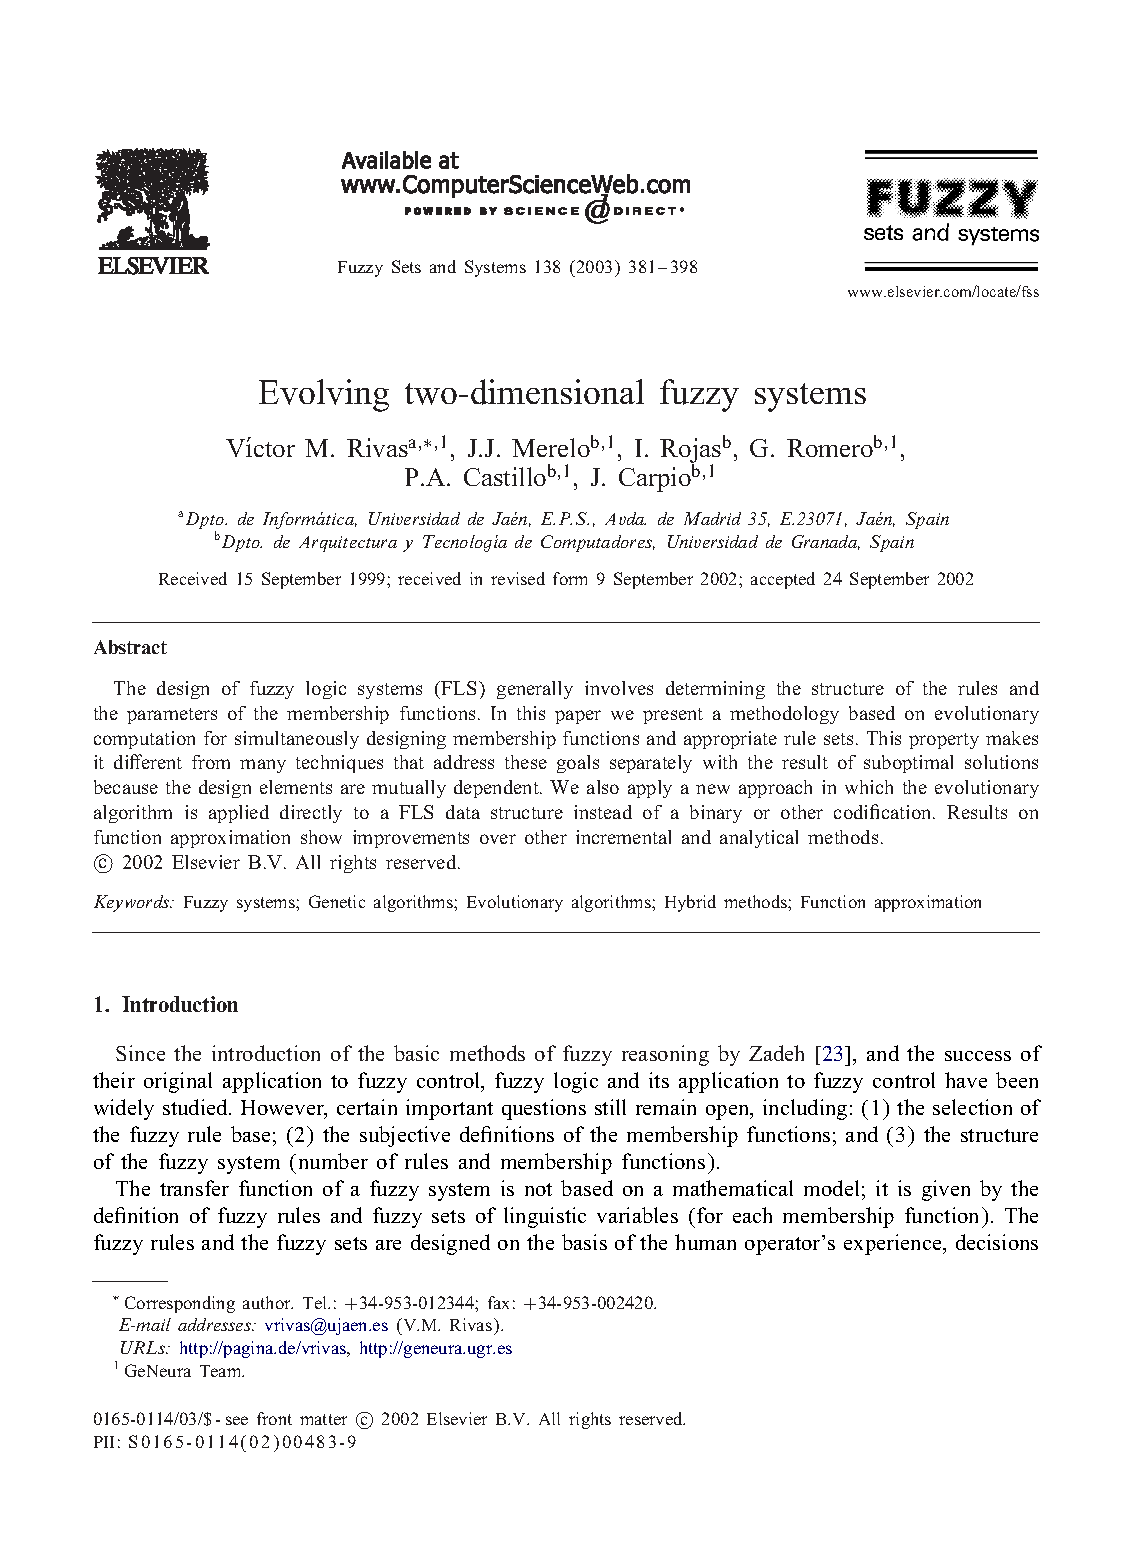
\includepdf[pages={-},scale=1.0,pagecommand={},offset=0 0,
addtolist={1, table, {Evolving two-dimensional fuzzy systems}, tab:evolving}]{pdf/evolving.pdf}
 
 % Página en blanco
 \newpage\null\thispagestyle{empty}\newpage
 
% ---- Artículo 2 

\section{From Classroom to Mobile Robots Competition Arena: ... } 

A continuaci\'on se detallan los datos del art\'iculo publicado relacionado con esta secci\'on de la disertaci\'on.\\
\\
T\'itulo: \textbf{From Classroom to Mobile Robots Competition Arena: An Experience on Artificial Intelligence Teaching}\\
Revista: \textbf{ The International journal of engineering education}, 2011; Factor de impacto: \textbf{0,418};\\
Autores: \textbf{Jos\'e Carpio Ca\~nada}, T. J. Mateo Sanguino, S. Alcocer, A. Borrego, A. Isidro, A. Palanco, J.M. Rodr\'iguez\\
\\
Relevancia de la revista:\\
\\
\begin{tabular}{ l c c c }
 \hline
  \fontsize{10}{12} \selectfont \specialcell{Nombre de la categor\'ia} & \fontsize{10}{12} \selectfont \specialcell{Revistas en\\la categor\'ia} & \fontsize{10}{12} \selectfont  \specialcell{Posici\'on en\\la categor\'ia} & \specialcell{Cuartil en\\la categor\'ia} \\
 \hline
  \fontsize{10}{12} \selectfont \specialcell{EDUCATION,\\ SCIENTIFIC DISCIPLINES} & 33 & 24 & Q4\\
  \fontsize{10}{12} \selectfont \specialcell{ENGINEERING,\\ MULTIDISCIPLINARY} & 90 & 60 & Q3 \\
   \hline
\end{tabular}




\setboolean{@twoside}{false}
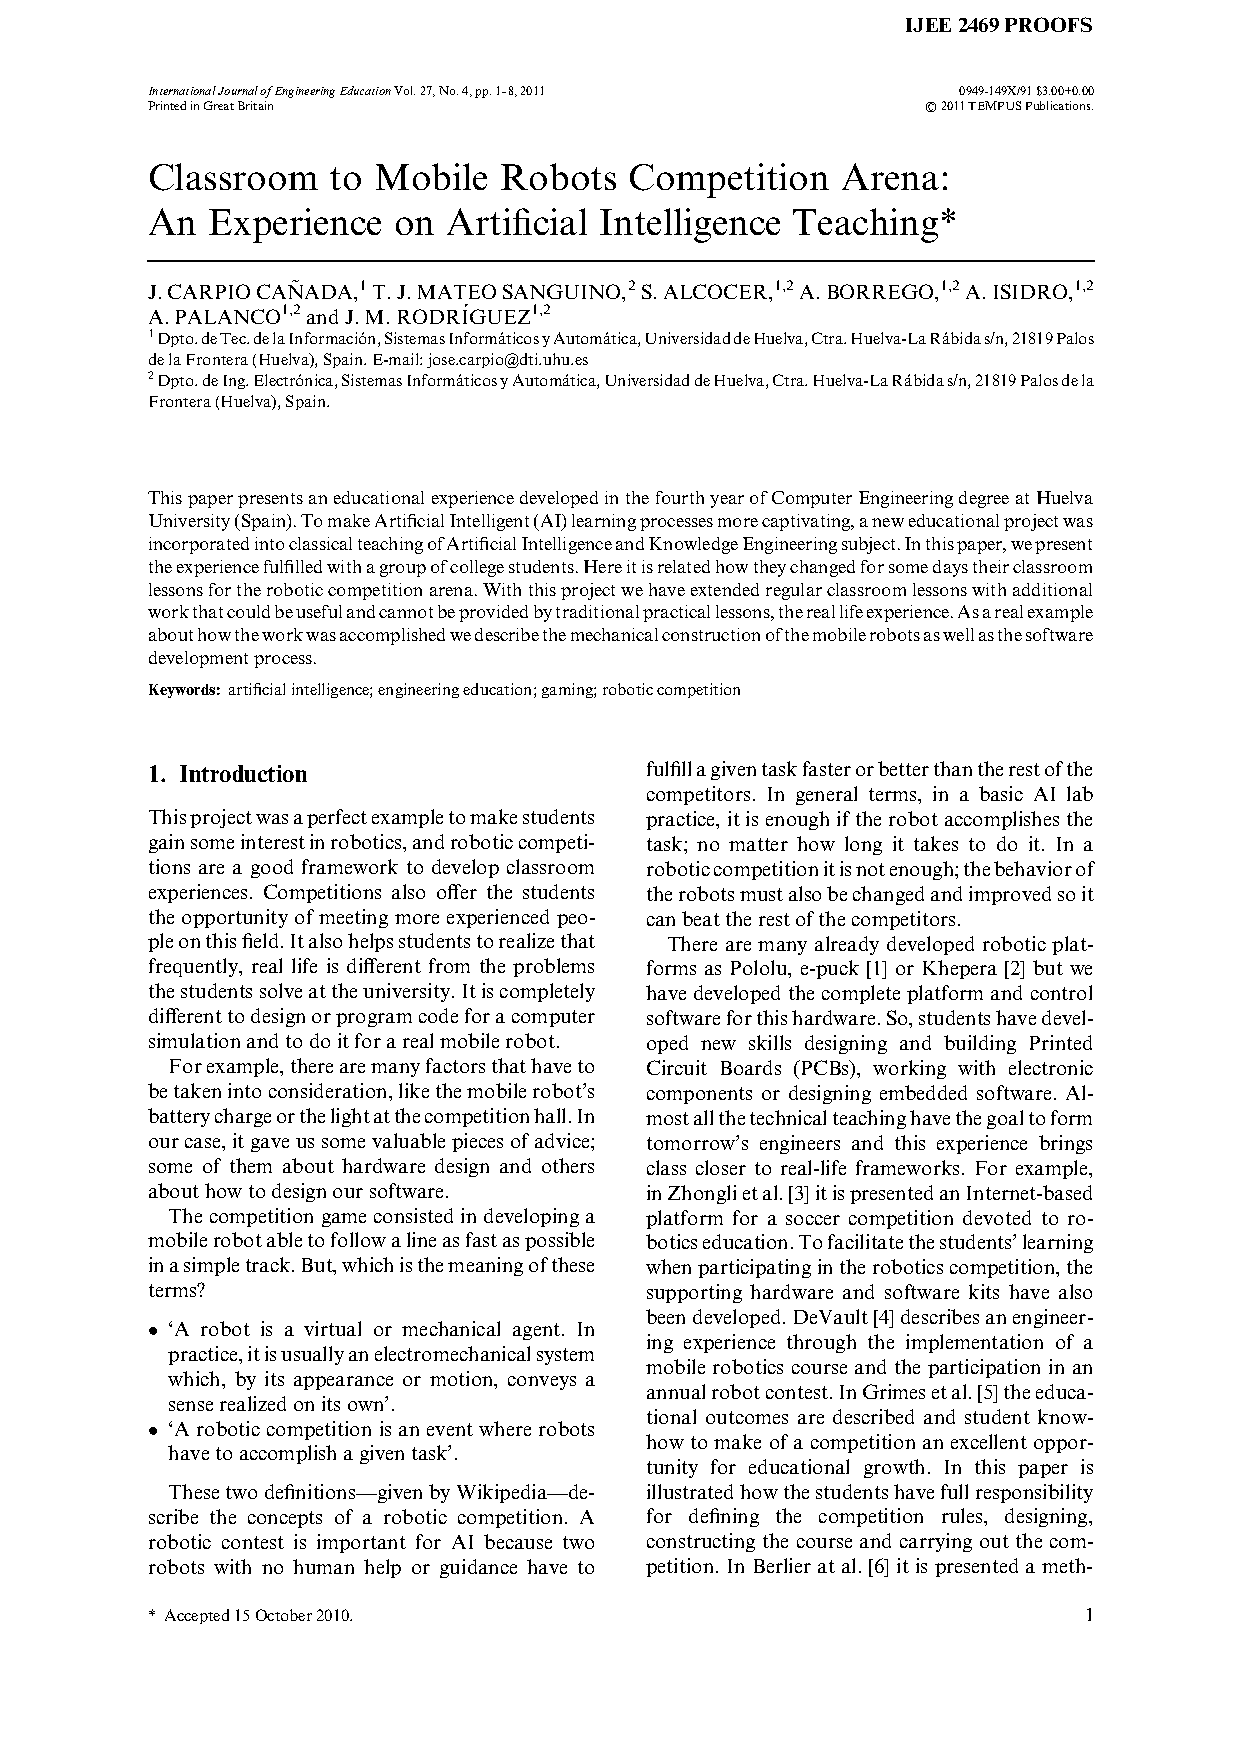
\includepdf[pages={-},scale=1.0,pagecommand={},offset=0 0,
addtolist={1, table, {From Classroom to Mobile Robots Competition Arena: An Experience on Artificial Intelligence Teaching}, tab:evolving}]{pdf/ijee2469ns.pdf} 
 
 % Página en blanco
 \newpage\null\thispagestyle{empty}\newpage
 
% ---- Artículo 3 

\section{Evolving the Strategies of Agents for the ANTS Game} 

A continuaci\'on se detallan los datos del art\'iculo publicado relacionado con esta secci\'on de la disertaci\'on.\\
\\
T\'itulo: \textbf{Evolving the Strategies of Agents for the ANTS Game}\\
Congreso: \textbf{International Work-Conference on Artificial Neural Networks (IWANN)}, 2013\\
Autores: \textbf{Jos\'e Carpio}, Pablo Garc\'ia-S\'anchez, Antonio Miguel Mora, Juan Juli\'an Merelo Guerv\'0s, Jes\'us Caraballo, Ferm\'in Vaz, Carlos Cotta\\
\\
Relevancia del congreso atendiendo al "Computer Science Conference Ranking"\\
\\
\begin{tabular}{ l c c }
 \hline
  \fontsize{10}{12} \selectfont Nombre del \'Area & \fontsize{10}{12} \selectfont  \specialcell{Posici\'on en\\la categor\'ia} \\
 \hline
  \fontsize{10}{12} \selectfont \specialcell{Artificial Intelligence\\ and Related Subjects} & \fontsize{10}{12} \selectfont Rank3\\
   \hline
\end{tabular}




\setboolean{@twoside}{false}
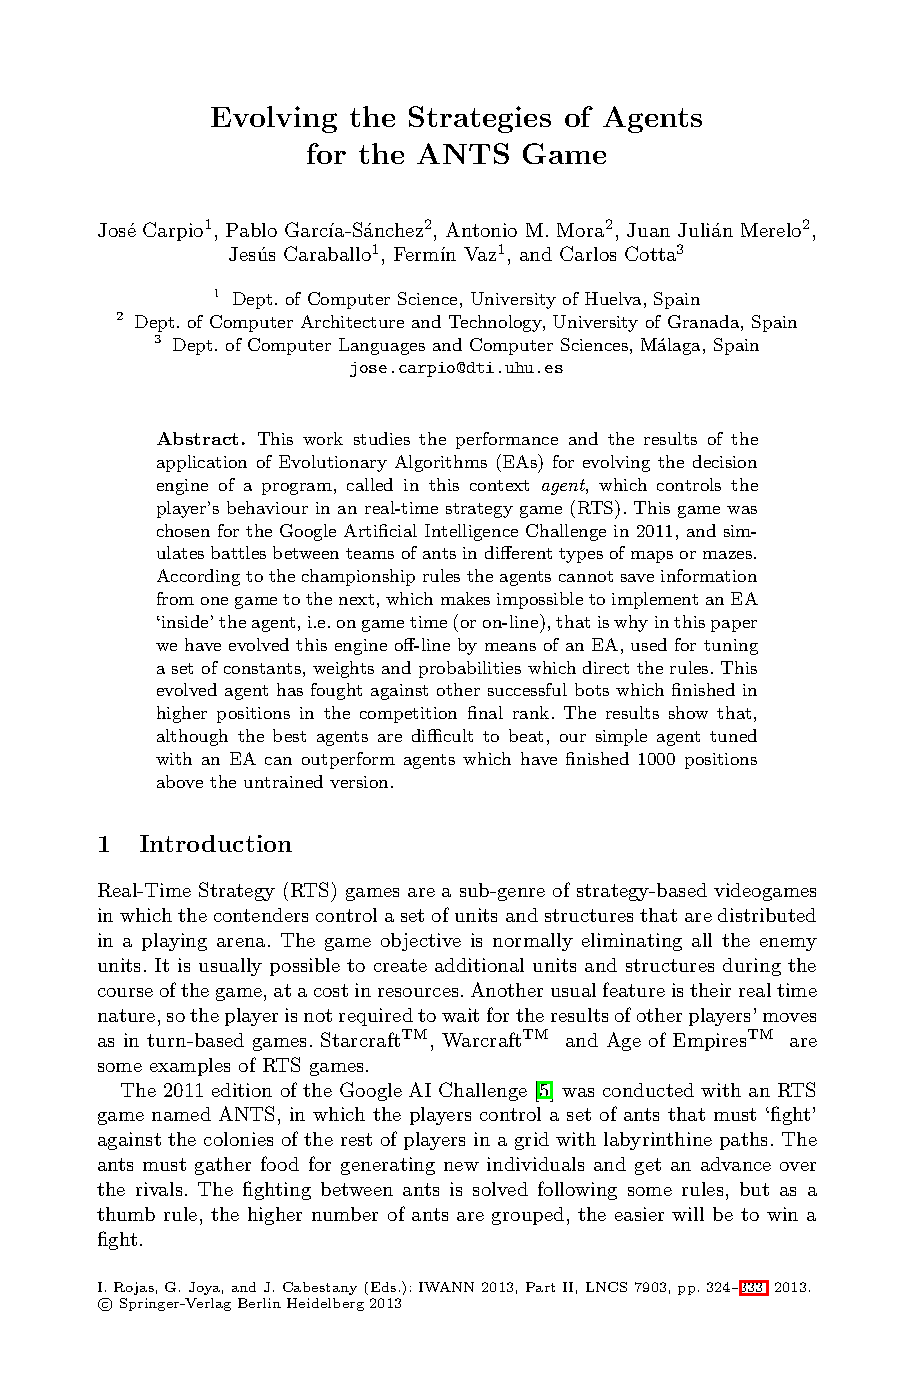
\includepdf[pages={-},scale=1.0,pagecommand={},offset=0 0,
addtolist={1, table, {Evolving the Strategies of Agents for the ANTS Game}, tab:evolving}]{pdf/ants_iwann2013.pdf}
 
 % Página en blanco
 \newpage\null\thispagestyle{empty}\newpage
 
% ---- Artículo 4 

\section{Open classroom: enhancing student achievement on artificial ...} 

T\'itulo: \textbf{Open classroom: enhancing student achievement on artificial intelligence through an international online competition}\\
Revista: \textbf{Journal of Computer Assisted Learning}, 2014; Factor de impacto: \textbf{1,023};\\
Autores: J. Carpio Ca\~nada, T.J. Mateo Sanguino, J.J. Merelo Guerv\'os, V.M. Rivas Santos\\
~\\
Relevancia de la revista:\\
~\\
\begin{tabular}{ l c c c }
 \hline
  \fontsize{10}{12} \selectfont \specialcell{Nombre de la categor\'ia} & \fontsize{10}{12} \selectfont \specialcell{Revistas en\\la categor\'ia} & \fontsize{10}{12} \selectfont  \specialcell{Posici\'on en\\la categor\'ia} & \specialcell{Cuartil en\\la categor\'ia} \\
 \hline
  \fontsize{10}{12} \selectfont \specialcell{EDUCATION\\ \& EDUCATIONAL RESEARCH} & 219 & 61 & Q2\\
   \hline
\end{tabular}




\setboolean{@twoside}{false}
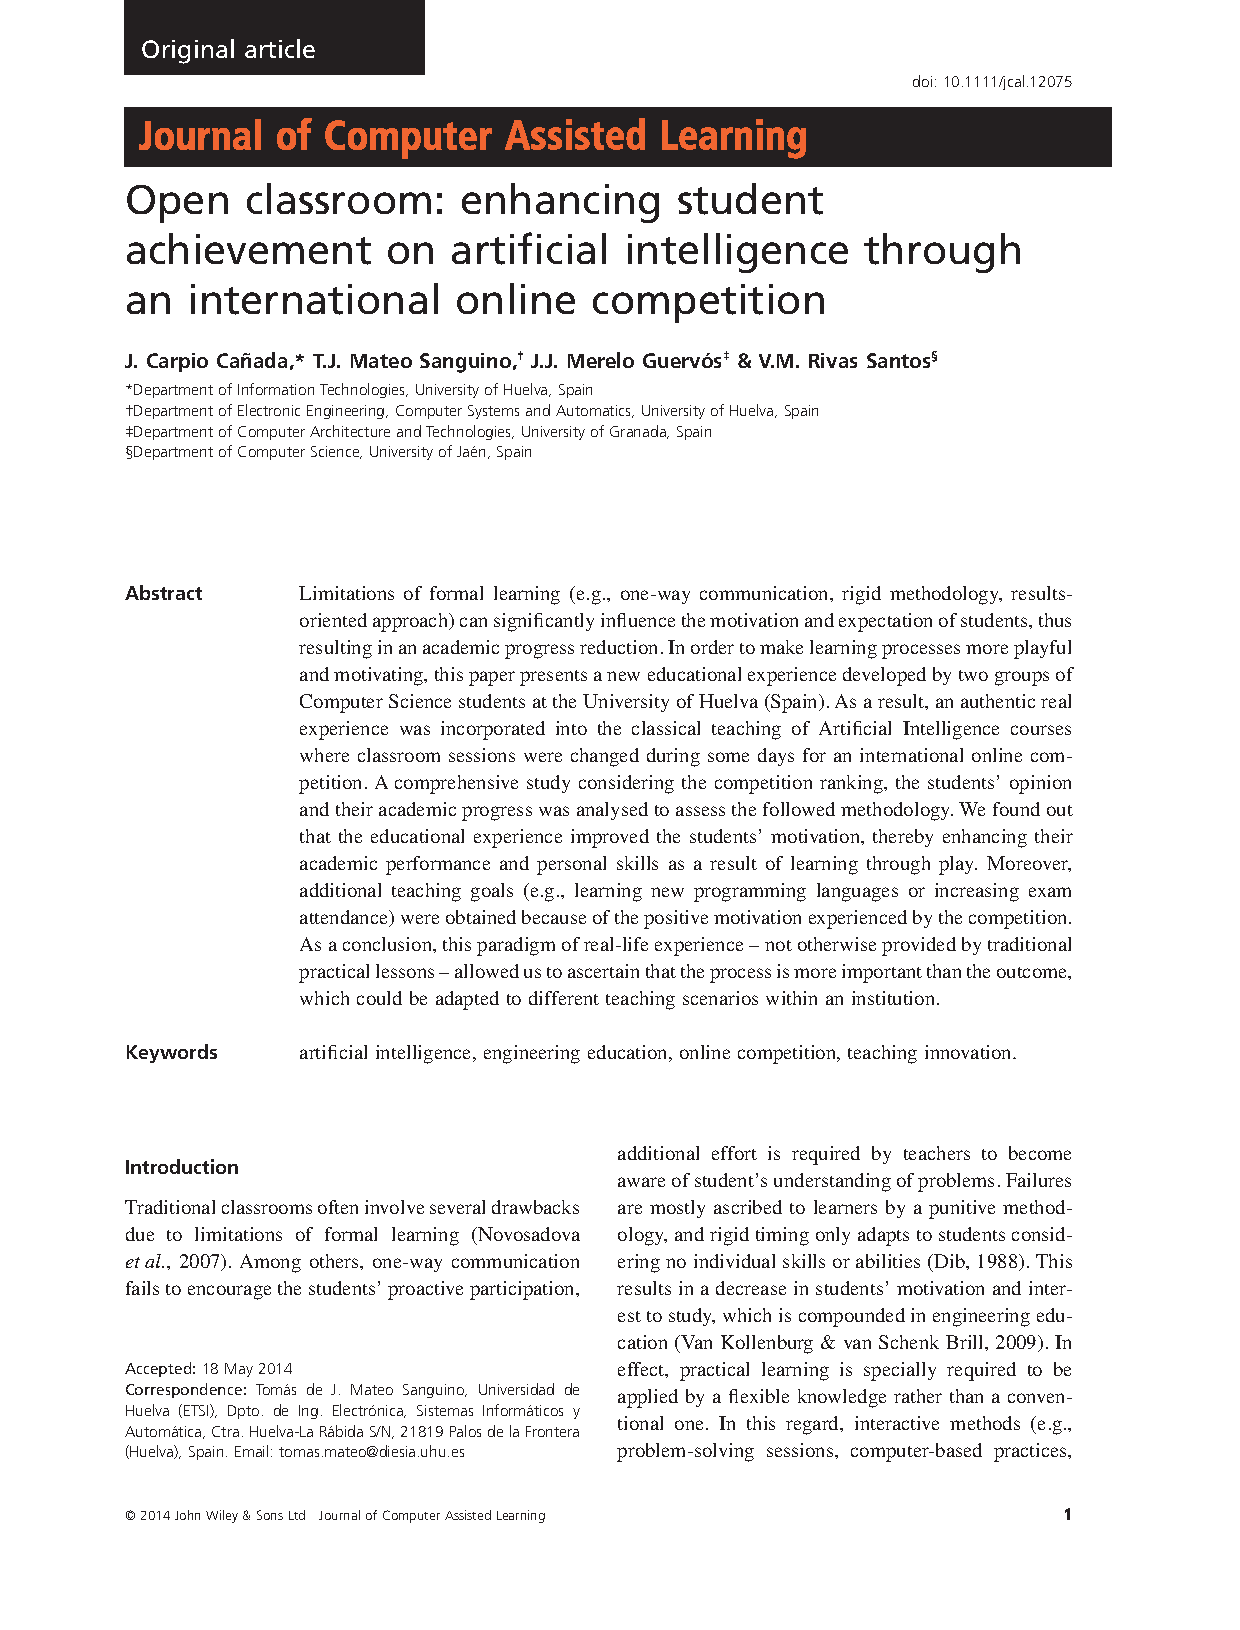
\includepdf[pages={-},scale=1.0,pagecommand={},offset=0 0,
addtolist={1, table, {Open classroom: enhancing student achievement on artificial intelligence through an international online competition}, tab:evolving}]{pdf/jcal12075.pdf}
 
  % Página en blanco
 \newpage\null\thispagestyle{empty}\newpage

% *******************************************************
% Backmatter
% *******************************************************
\appendix
\myPart{Ap\'endice}
% \include{Chapters/appendixosgi}
% \include{Chapters/appendixosgiliath}


%\include{Chapters/apendiceC}
%********************************************************************
% Other Stuff in the Back
%*******************************************************
\cleardoublepage
%********************************************************************
% Bibliography
%*******************************************************
% work-around to have small caps also here in the headline
\pdfbookmark[0]{\bibname}{\bibname}

% \manualmark
% \markboth{\spacedlowsmallcaps{\bibname}}{\spacedlowsmallcaps{\bibname}} % work-around to have small caps also
%\phantomsection
\refstepcounter{dummy}
\addtocontents{toc}{\protect\vspace{\beforebibskip}} % to have the bib a bit from the rest in the toc
\addcontentsline{toc}{chapter}{\tocEntry{\bibname}}
%\bibliographystyle{plainnat}
\bibliographystyle{babplain-fl}
\label{app:bibliography}
\bibliography{tesis} 
%\cleardoublepage
%%*******************************************************
% Declaration
%*******************************************************
\refstepcounter{dummy}
\pdfbookmark[1]{Declaraci�n}{Declaraci�n}
\chapter*{Declaraci�n}
\thispagestyle{empty}
\vfill

\noindent El doctorando \myName y los directores de la tesis \myDirectorOne y \myDirectorTwo \xspace garantizamos, al firmar esta tesis doctoral, que el trabajo ha sido realizado por el doctorando bajo la direcci�n de los directores de la tesis y hasta donde nuestro conocimiento alcanza, en la realizaci�n del trabajo, se han respetado los derechos de otros autores a ser citados, cuando se han utilizado sus resultados o publicaciones.  
\smallskip


\bigskip

\noindent\textit{\myLocation, \myTime}

\bigskip
\bigskip
\bigskip

\begin{flushright}
    \begin{tabular}{m{3cm}m{7cm}}
        & \\ \hline
        \centering\myName & \myDirectorOne \newline y \myDirectorTwo
    \end{tabular}
\end{flushright}

\vfill
\cleardoublepage
%La contraportada tiene que estar en página par!!
% \include{FrontBackmatter/DirtyBackpage}

% ********************************************************************
% Game Over: Restart, Restore or Quit?
%*******************************************************
\listoftodos[Notes]
\end{document}
% ********************************************************************
